\documentclass[11pt,a4paper]{article}

% Packages
\usepackage[utf8]{inputenc}
\usepackage[greek,english]{babel}
\usepackage{alphabeta}
\usepackage[margin=1in]{geometry}
\usepackage{amsmath,amssymb,amsthm}
\usepackage{graphicx}
\usepackage{float}
\usepackage{hyperref}
\usepackage{listings}
\usepackage{xcolor}
\usepackage{booktabs}
\usepackage[autostyle, english = american]{csquotes}
\MakeOuterQuote{"}
\usepackage{caption}
\usepackage{subcaption}
\usepackage{verbatim}

% Hyperref setup
\hypersetup{
    colorlinks=true,
    linkcolor=blue,
    filecolor=magenta,      
    urlcolor=cyan,
    citecolor=blue
}

% Code listing setup
\definecolor{codegreen}{rgb}{0,0.6,0}
\definecolor{codegray}{rgb}{0.5,0.5,0.5}
\definecolor{codepurple}{rgb}{0.58,0,0.82}
\definecolor{backcolour}{rgb}{0.95,0.95,0.92}

\lstdefinestyle{mystyle}{
    backgroundcolor=\color{backcolour},   
    commentstyle=\color{codegreen},
    keywordstyle=\color{magenta},
    numberstyle=\tiny\color{codegray},
    stringstyle=\color{codepurple},
    basicstyle=\ttfamily\footnotesize,
    breakatwhitespace=false,         
    breaklines=true,                 
    captionpos=b,                    
    keepspaces=true,                 
    numbers=left,                    
    numbersep=5pt,                  
    showspaces=false,                
    showstringspaces=false,
    showtabs=false,                  
    tabsize=2
}
\lstset{style=mystyle}

% Title information
\title{\textbf{Εργαστήριο 1} \\ \bigskip
\large Αναγνώριση φωνής με Κρυφά Μαρκοβιανά Μοντέλα και Αναδρομικά Νευρωνικά Δίκτυα}
\author{Κόρδας Νικόλαος (03121032) \\
        Κριθαρίδης Κωνσταντίνος (03121045) \\
        }
\date{\today}

\begin{document}

\maketitle

\section*{Περιγραφή}

\subsection*{Ο μηχανισμός παραγωγής φωνής}

\textbf{Φωνητική οδός (\foreignlanguage{english}{vocal tract}):} Πρόκειται για τη σειρά των οργάνων στον ανθρώπινο λαιμό και το κεφάλι που συνδέονται με την παραγωγή ήχου, από το λάρυγγα μέχρι τα χείλη και τη μύτη. Ο αρχικός ήχος παράγεται από την δόνηση των φωνητικών χορδών στον λάρυγγα. 
Ο ήχος ταξιδεύει μέσω της φωνητικής οδού. Το φάσμα της φωνής διαμορφώνεται από τη συχνοτική επιλεκτικότητα της φωνητικής οδού. \\

\noindent \textbf{\foreignlanguage{english}{Formants}:} Οι συχνότητες συντονισμού του φωνητικού σωλήνα ονομάζονται \foreignlanguage{english}{formants}. \\
\noindent Όταν μετράμε τα \foreignlanguage{english}{formants} για τα φωνήεντα α, ου, ι, στην πραγματικότητα μετράμε τις συχνότητες συντονισμού του φωνητικού σωλήνα για το καθένα τους. Δεδομένου ότι ο φωνητικός σωλήνας των ανδρών είναι γενικά μεγαλύτερος από αυτόν των γυναικών, τα formants του ομιλητή 1 αναμένονται σε χαμηλότερες συχνότητες. \\

\noindent \textbf{\foreignlanguage{english}{Pitch}:} Είναι η θεμελιώδης συχνότητα ταλάντωσης των φωνητικών χορδών κατά την παραγωγή του ήχου. Συνήθως, είναι χαμηλότερη στους άνδρες ενώ επηρεάζεται από το συναισθηματισμό, το τόνο και την προσωδία της ομιλίας. \cite{RabinerSchafer1978} \\


\section*{Βήμα 1}

Χρησιμοποιούμε το praat για να αναλύσουμε τα σήματα ήχου μας και να εξάγουμε τις πληροφορίες που ζητούνται στην εκφώνηση.

\subsection*{Αρχείο onetwothree1.wav}

Ανοίγουμε το αρχείο στο praat για να κάνουμε annotations στα φωνήματα που μας ενδιαφέρουν. Έτσι, ορίζουμε ταυτόχρονα τις περιοχές όπου θα εξάγουμε το μέσο pitch. Πιο συγκεκριμένα, για αυτόν τον ομιλητή έχουμε ότι (από τα αρχεία που παράγει το praat): 

\begin{itemize}
	\item \textbf{Pitch (α):} 134.30091712757704 Hz (mean pitch in SELECTION)
	\item \textbf{Pitch (ου):} 130.34836851658105 Hz (mean pitch in SELECTION)
	\item \textbf{Pitch (ι):} 133.11983451151906 Hz (mean pitch in SELECTION)
\end{itemize}

\noindent Αντίστοιχα, από το αρχείο για τα formants:
      
\begin{itemize}
	\item \textbf{Φώνημα α:}
		\begin{itemize}
			\item \textbf{F1\_Hz:} 639.117504
			\item \textbf{F2\_Hz:} 3014.697815
			\item \textbf{F3\_Hz:} 3787.044970
		\end{itemize}
		
	\item \textbf{Φώνημα ου:}
		\begin{itemize}
			\item \textbf{F1\_Hz:} 507.160260
			\item \textbf{F2\_Hz:} 2086.948531
			\item \textbf{F3\_Hz:} 3522.142285 
		\end{itemize}
	
	\item \textbf{Φώνημα ι:}
		\begin{itemize}
			\item \textbf{F1\_Hz:} 326.202470
			\item \textbf{F2\_Hz:} 2250.289657
			\item \textbf{F3\_Hz:} 3421.036991
		\end{itemize}
\end{itemize}

\noindent Παρακάτω δίνουμε ένα στιγμιότυπο της διαδικασίας της επεξεργασίας και εξαγωγής των πληροφοριών:

\begin{figure}[H]
    \centering
    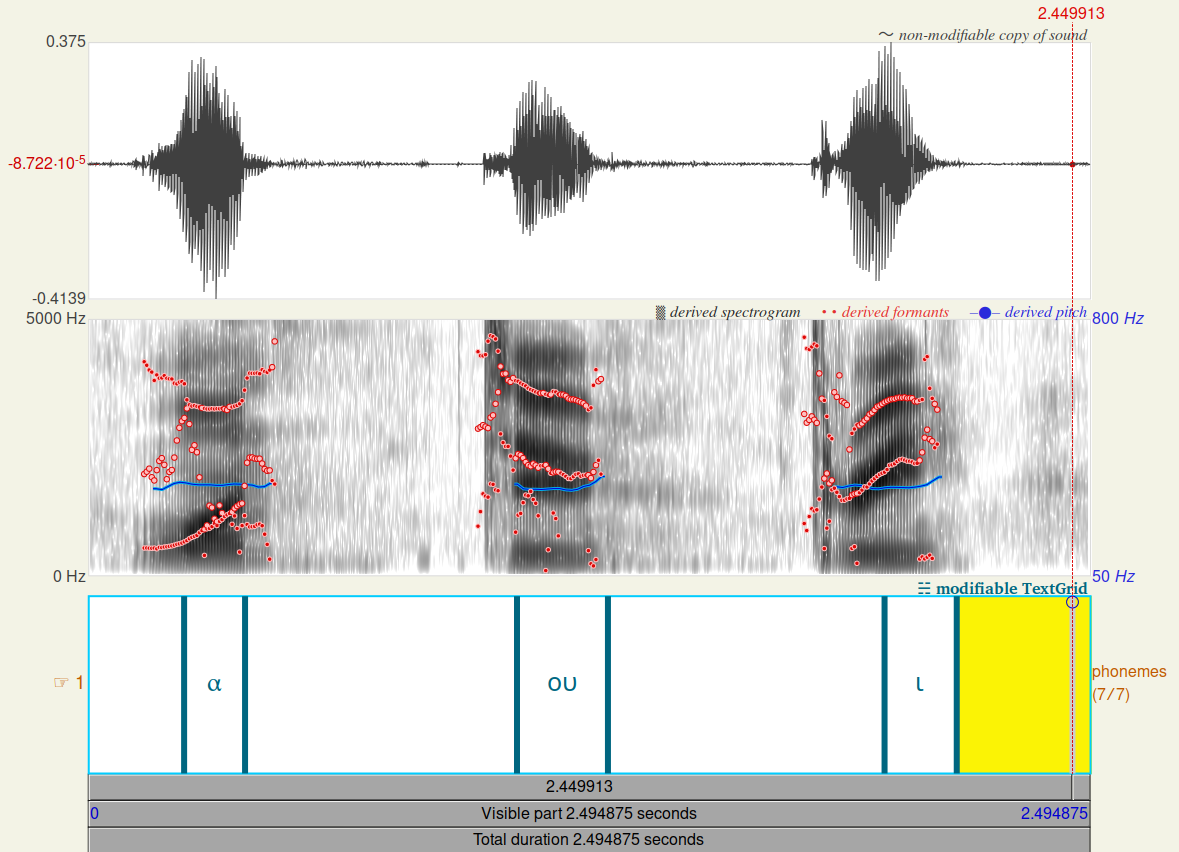
\includegraphics[width=0.6\linewidth]{plots/onetwothree1_praat.png}
\end{figure}

\noindent Τέλος σχεδιάσαμε τα παρακάτω διαγράμματα που οπτικοποιούν την εργασία μας (1ο) και τις μετρήσεις μας (2ο)

\begin{figure}[H]
    \centering
    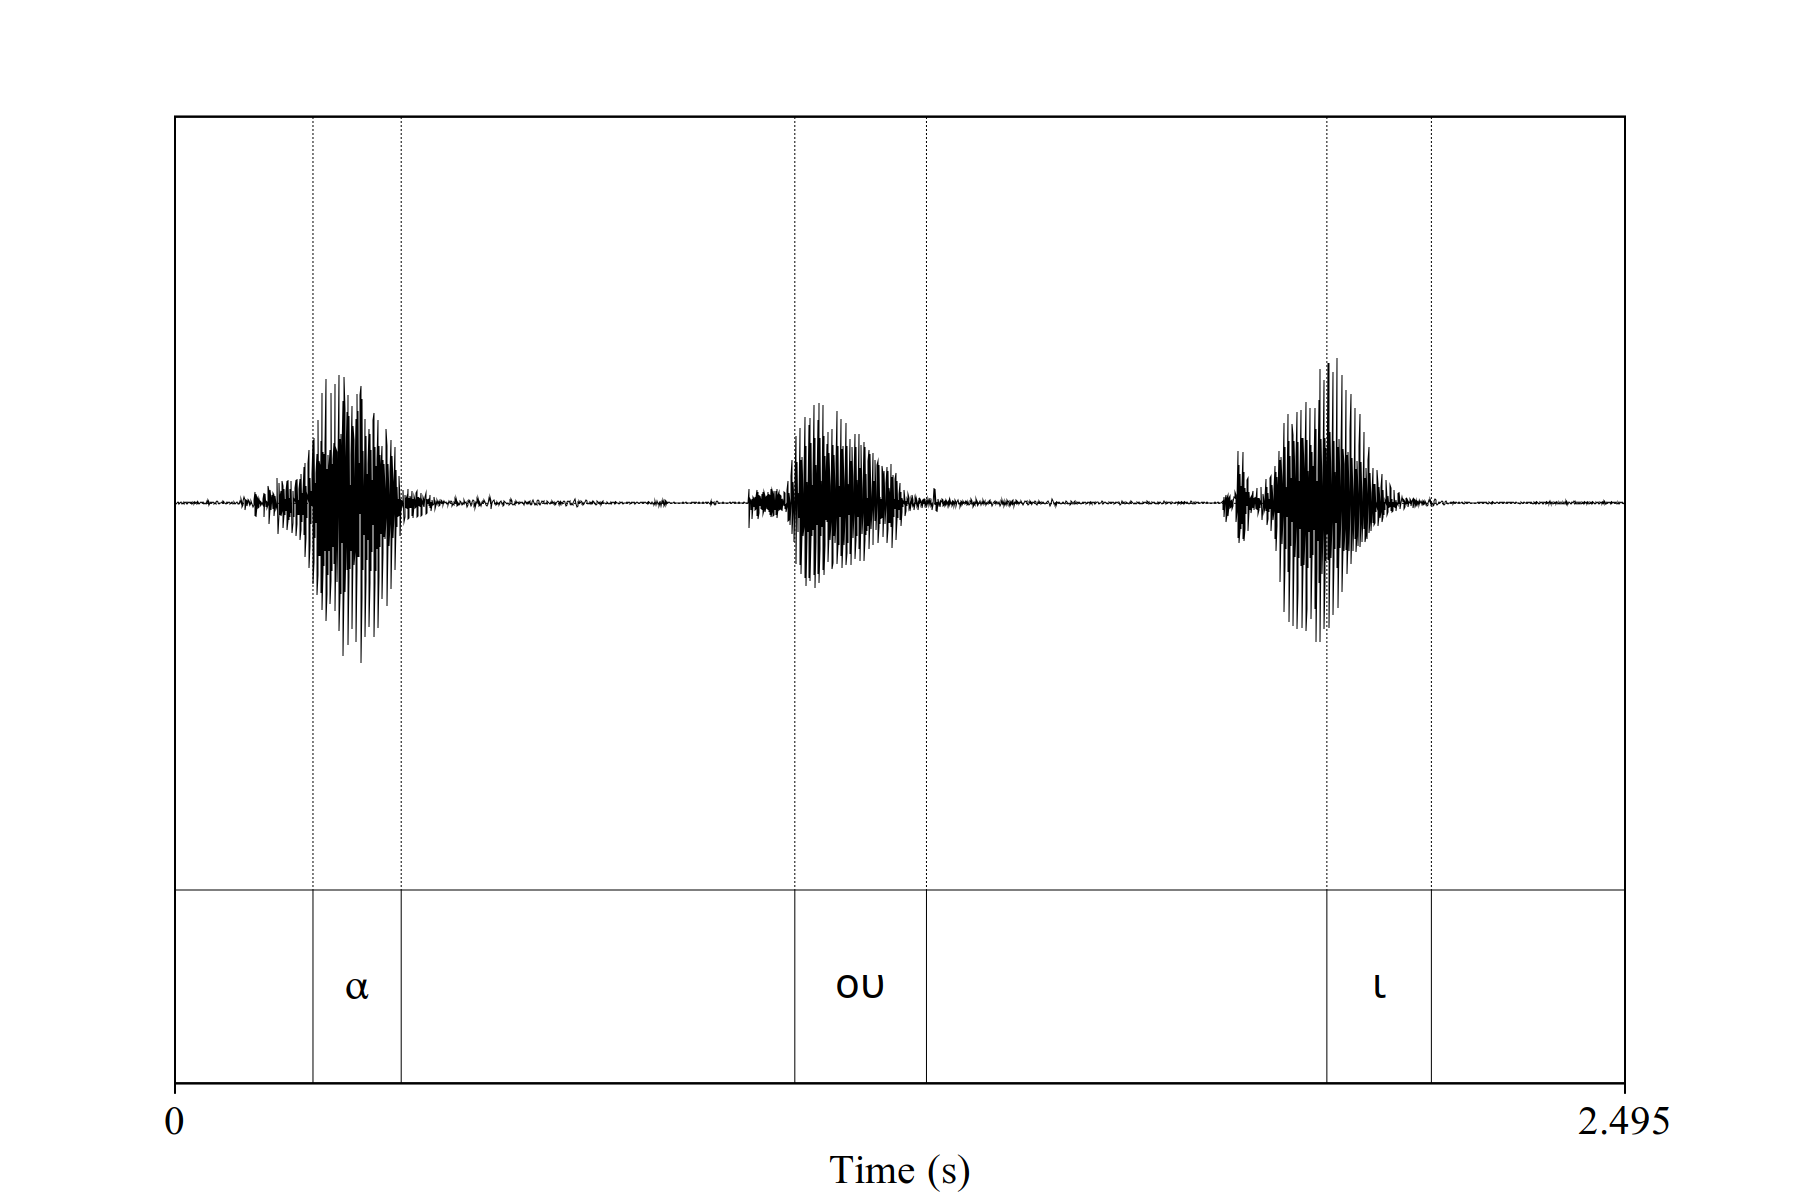
\includegraphics[width=0.6\linewidth]{plots/onetwothree1_annot.png}
\end{figure}

\begin{figure}[H]
    \centering
    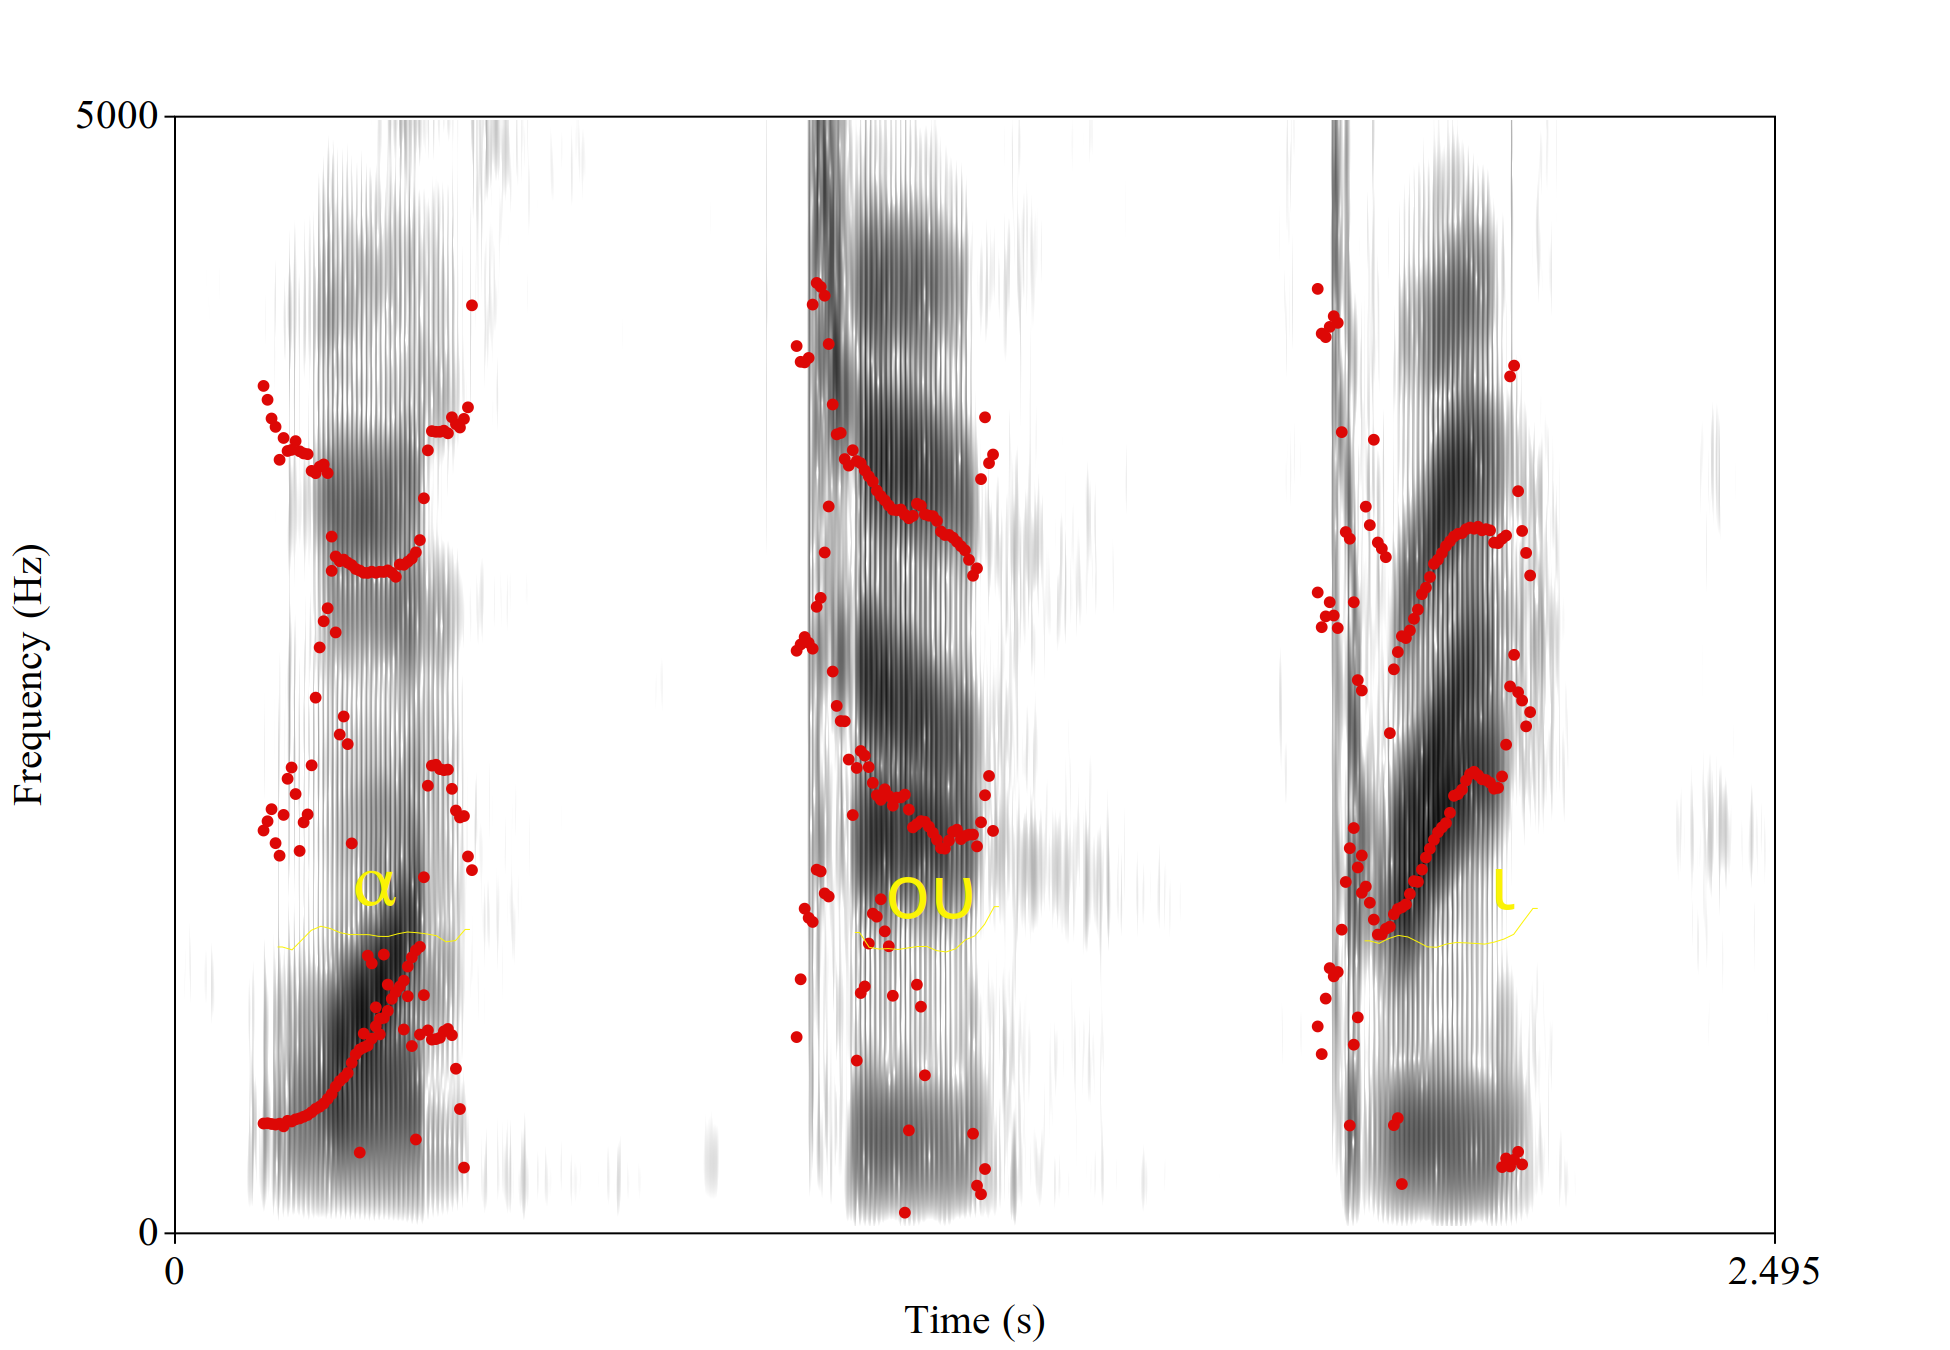
\includegraphics[width=0.7\linewidth]{plots/spectrogram_pitch_formants1.png}
\end{figure}

\subsection*{Αρχείο onetwothree8.wav}

Αντίστοιχα με το προηγούμενο αρχείο οι μετρήσεις μας για το pitch κάθε φωνήματος είναι:

\begin{itemize}
	\item \textbf{Pitch (α):} 178.90096253179337 Hz (mean pitch in SELECTION)
	\item \textbf{Pitch (ου):} 183.19462142657264 Hz (mean pitch in SELECTION)
	\item \textbf{Pitch (ι):} 176.88367983435367 Hz (mean pitch in SELECTION)
\end{itemize}

\noindent Για τα formants:

\begin{itemize}
	\item \textbf{Φώνημα α:}
		\begin{itemize}
			\item \textbf{F1\_Hz:} 674.367922
			\item \textbf{F2\_Hz:} 703.507187
			\item \textbf{F3\_Hz:} 4112.994619 
		\end{itemize}
		
	\item \textbf{Φώνημα ου:}
		\begin{itemize}
			\item \textbf{F1\_Hz:} 376.486131
			\item \textbf{F2\_Hz:} 2801.849314
			\item \textbf{F3\_Hz:} 3860.898207
		\end{itemize}
	
	\item \textbf{Φώνημα ι:}
		\begin{itemize}
			\item \textbf{F1\_Hz:} 345.351842 
			\item \textbf{F2\_Hz:} 2549.549245 
			\item \textbf{F3\_Hz:} 3396.739966
		\end{itemize}
\end{itemize}

\noindent Τα αντίστοιχα διαγράμματα είναι:

\begin{figure}[H]
    \centering
    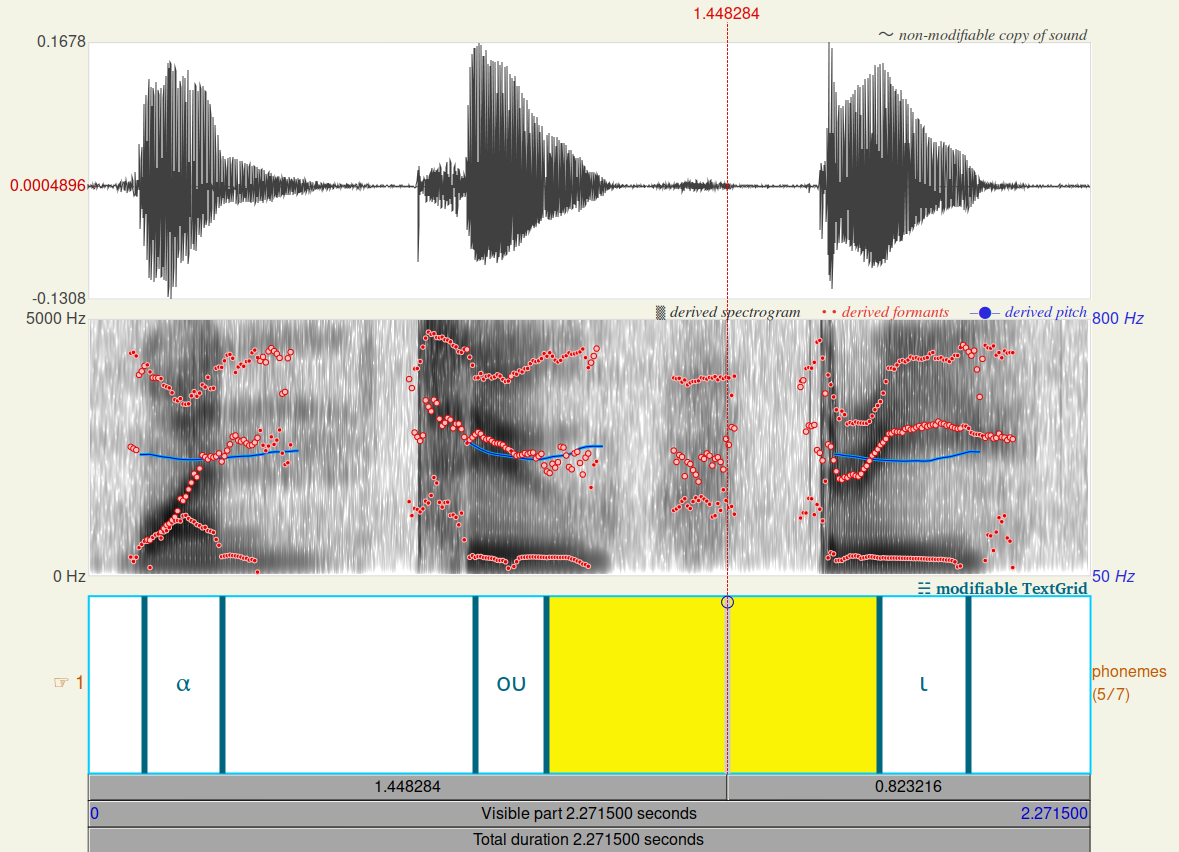
\includegraphics[width=0.5\linewidth]{plots/onetwothree8.png}
\end{figure}

\begin{figure}[H]
    \centering
    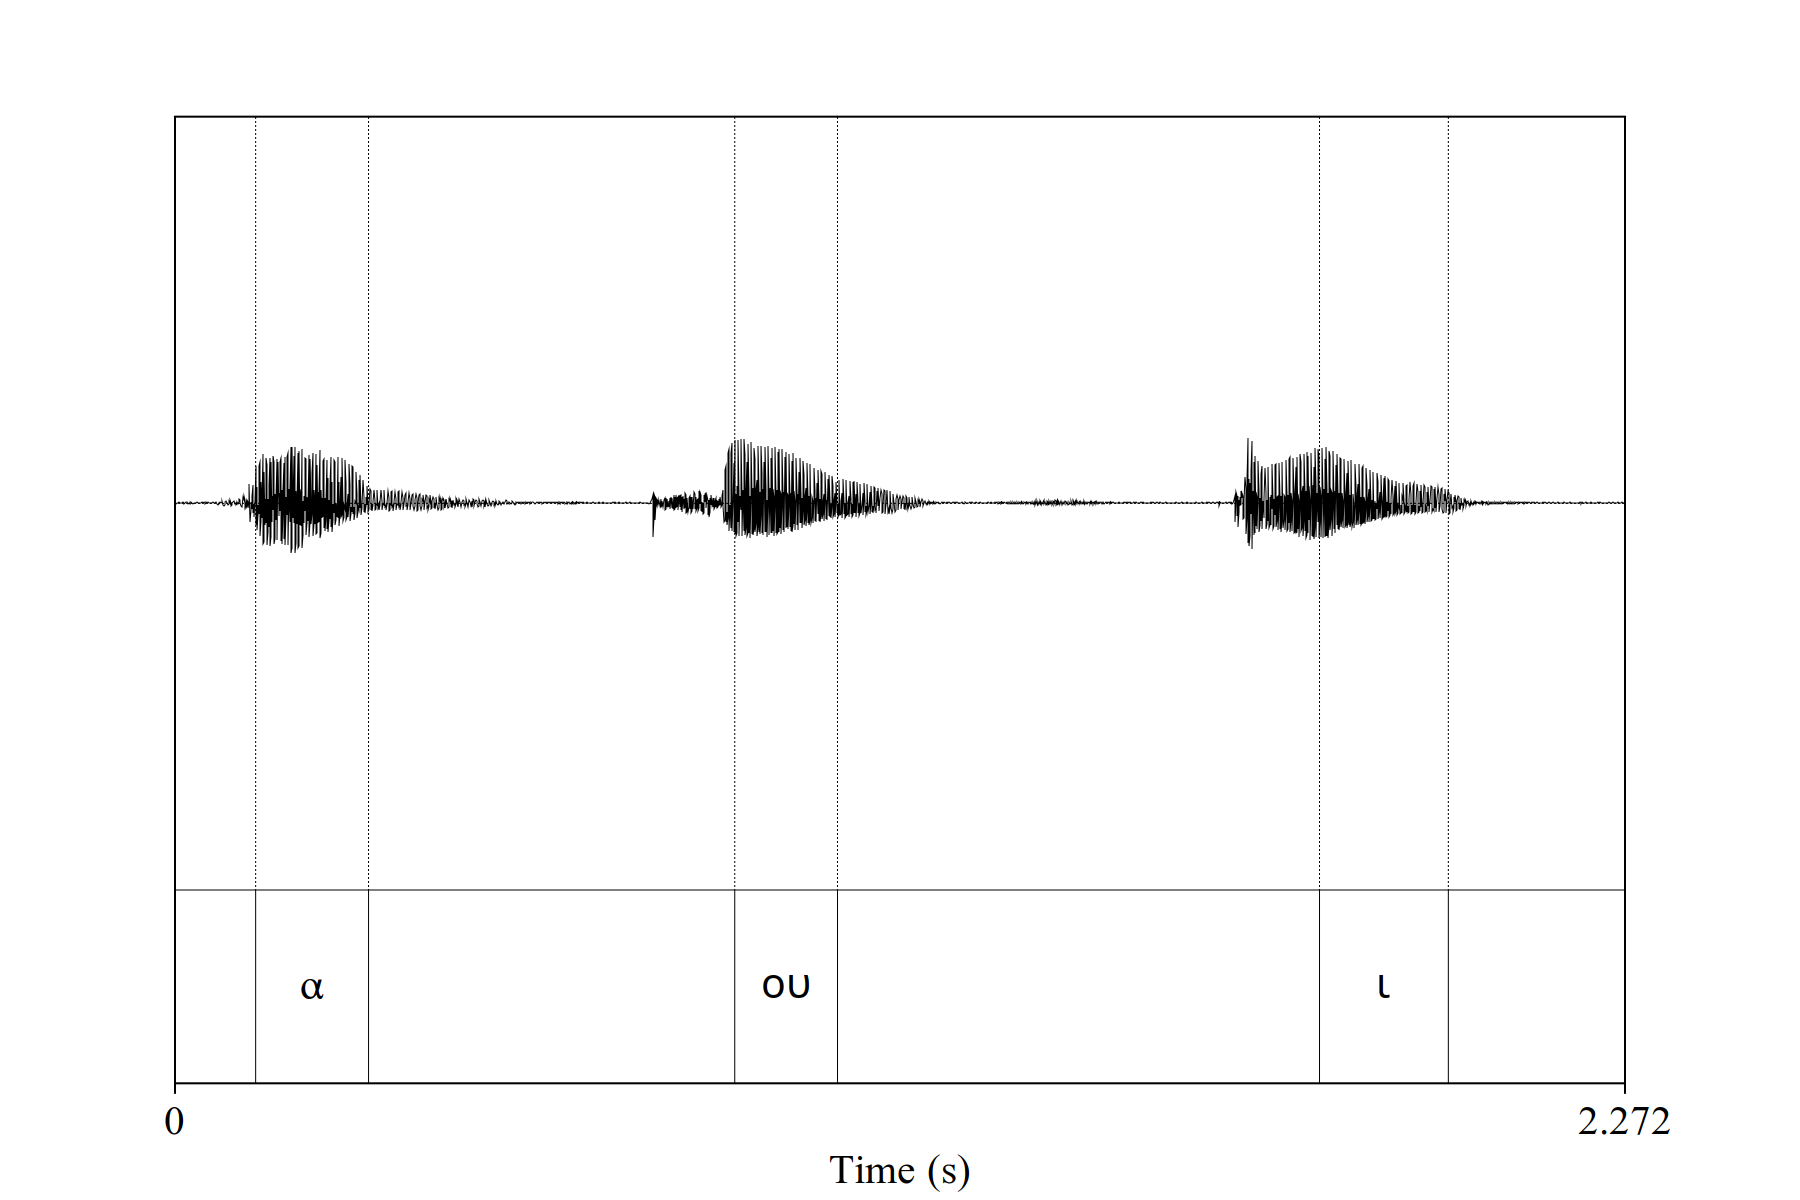
\includegraphics[width=0.55\linewidth]{plots/onetwothree8_annot.png}
\end{figure}

\begin{figure}[H]
    \centering
    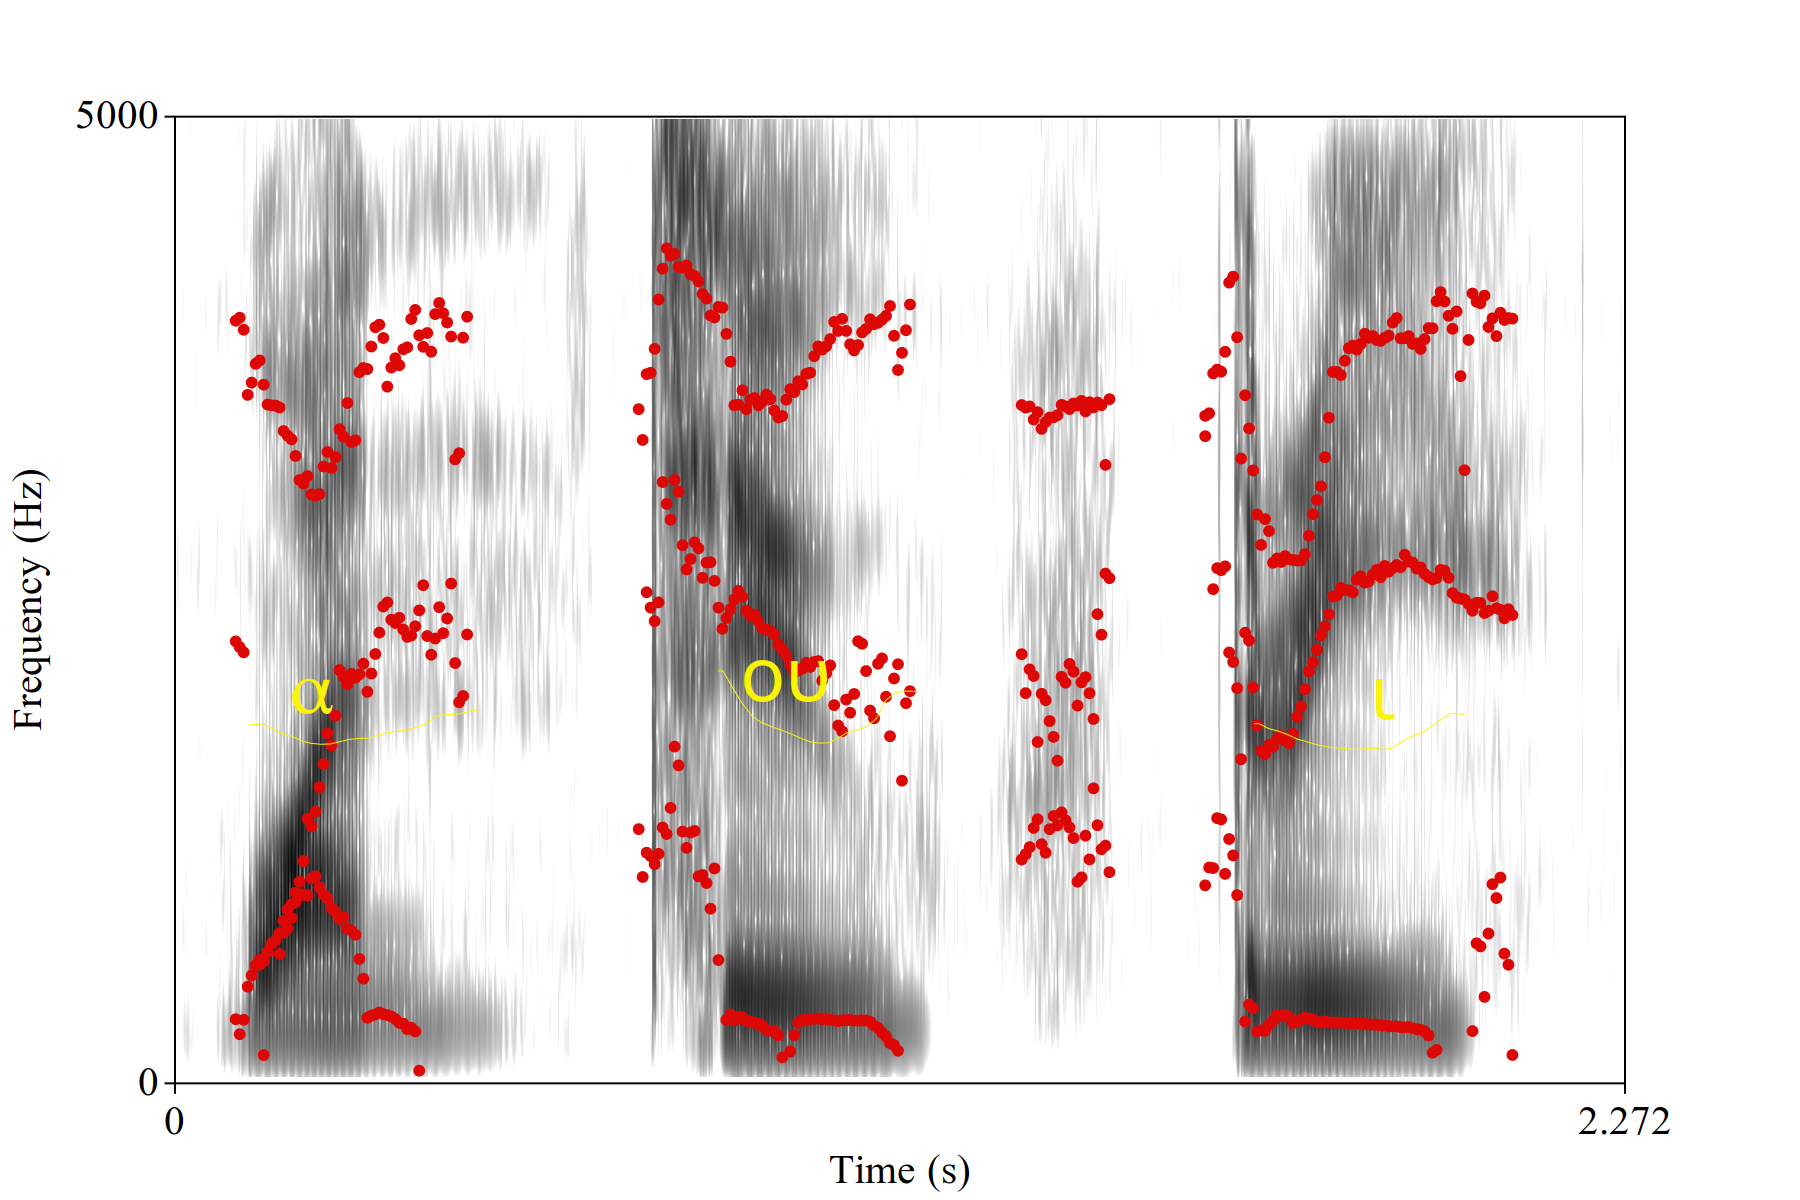
\includegraphics[width=0.55\linewidth]{plots/onetwothree8_info.png}
\end{figure}

\subsection*{Συμπεράσματα}
Βλέπουμε πως οι μετρήσεις μας συμφωνούν απόλυτα με τις θεωρητικές προσδοκίες που αναφέρθηκαν στην περιγραφή παραπάνω. Πιο συγκεκριμένα, τα pitch (μέσες τιμές) της γυναίκας (αρχείο onetwothree8.wav) βρίσκονται σε υψηλότερες συχνότητες από τις αντίστοιχες του άντρα. \\

\noindent Επιπλέον, κατά κανόνα τα formants του άντρα βρίσκονται σε χαμηλότερες συχνότητες αντανακλώντας τα διαφορετικά φυσικά χαρακτηριστικά της φωνητικής του οδού (είναι μεγαλύτερη).
    
\section*{Βήμα 2}

Στο βήμα αυτό ξεκινάει ο κώδικάς μας σε Python 3.

\noindent Ξεκινάμε γράφοντας την συνάρτηση data\_parser που σκανάρει τον φάκελο \verb|pr_lab2_data / digits| και επιστρέφει τρεις λίστες που περιέχουν τα δεδομένα των αρχείων wav, το id των ομιλητών και το ψηφίο που εκφωνούν, αντίστοιχα. 

\noindent Τα δεδομένα του αρχείου wav τα φορτώνουμε με τη συνάρτηση load της βιβλιοθήκης librosa, τα ids των ομιλητών με την μέθοδο isdigit() των strings, και τα ψηφία με την μέθοδο isalpha() στο τμήμα του filename πριν την κατάληξη.

\lstinputlisting[language=Python, firstline=26, lastline=44]{preparation.py}

\noindent Στην συνάρτηση main καλούμε την συνάρτηση data\_parser που μόλις γράψαμε ως εξής:

\lstinputlisting[language=Python, firstline=829, lastline=831]{preparation.py}

\noindent Στο τέλος, όπως φαίνεται στον κώδικα παραπάνω, κάνουμε μία ανάλυση των στατιστικών των ψηφίων.

\begin{figure}[H]
    \centering
    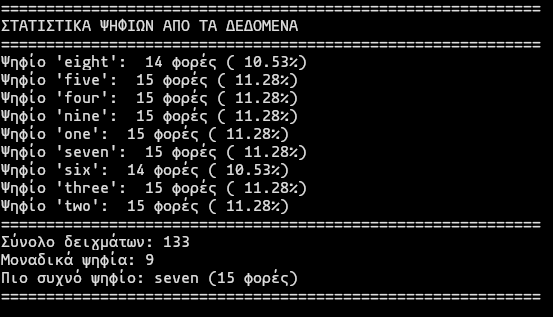
\includegraphics[width=0.55\linewidth]{plots/digits_stats.png}
\end{figure}

\noindent Αυτό το κάνουμε για να εξετάσουμε αν το dataset είναι ισορροπημένο ή όχι και αν όχι προς τα πού είναι biased. Όπως βλέπουμε, όμως, το dataset είναι ισορροπημένο. Έτσι, το accuracy θα είναι μία καλή μετρική για την αξιολόγηση των ταξινομητών που θα εκπαιδεύσουμε στη συνέχεια της εργασίας.

\section*{Βήμα 3}

Στο βήμα αυτό εξάγουμε τα Mel-frequency cepstral coefficients (MFCCs) των σημάτων. Οι συντελεστές αυτοί προκύπτουν από Discrete Cosine Transform εφαρμοσμένο στον λογάριθμο της φασματικής πυκνότητας ισχύος ειλημμένη στην κλίμακα mel ώστε ισαπέχοντα διαστήματα συχνοτήτων να ακούγονται εξίσου μακριά στο ανθρώπινο αυτί. Η διαφορά στην κλίμακα είναι που την διαφοροποιεί από το κανονικό cepstrum, του οποίο η διαδικασία παριστάνεται και γραφικά στο παρακάτω διάγραμμα του \cite{RabinerSchafer1978}.

\begin{figure}[H]
    \centering
    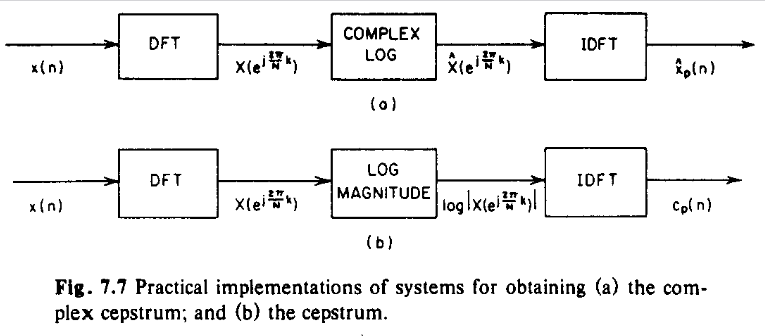
\includegraphics[width=0.7\linewidth]{plots/cepstrum.png}
\end{figure}

\noindent Χρησιμοποιούμε παράθυρο μήκους 25ms, βήμα 10ms και εξάγουμε ως χαρακτηριστικά τα 13 MFCCs ανά αρχείο. Επιπλέον, υπολογίζουμε την πρώτη και δεύτερη διακριτή παράγωγο των MFCCs κατά την μετακίνηση του παραθύρου λήψης τους. Η βιβλιοθήκη librosa έχει συναρτήσεις για όλα αυτά τα ζητούμενα, οπότε η τελική συνάρτηση και η κλήση της στη main φαίνονται παρακάτω:

\lstinputlisting[language=Python, firstline=73, lastline=87]{preparation.py}

\lstinputlisting[language=Python, firstline=833, lastline=834]{preparation.py}

\section*{Βήμα 4}

Αρχικά, δημιουργούμε ιστογράμματα για το 1ο και 2ο MFCC για όλες τις εκφωνήσεις των ψηφίων $n_1 = 2$ και $n_2 = 5$.

\begin{figure}[H]
    \centering
    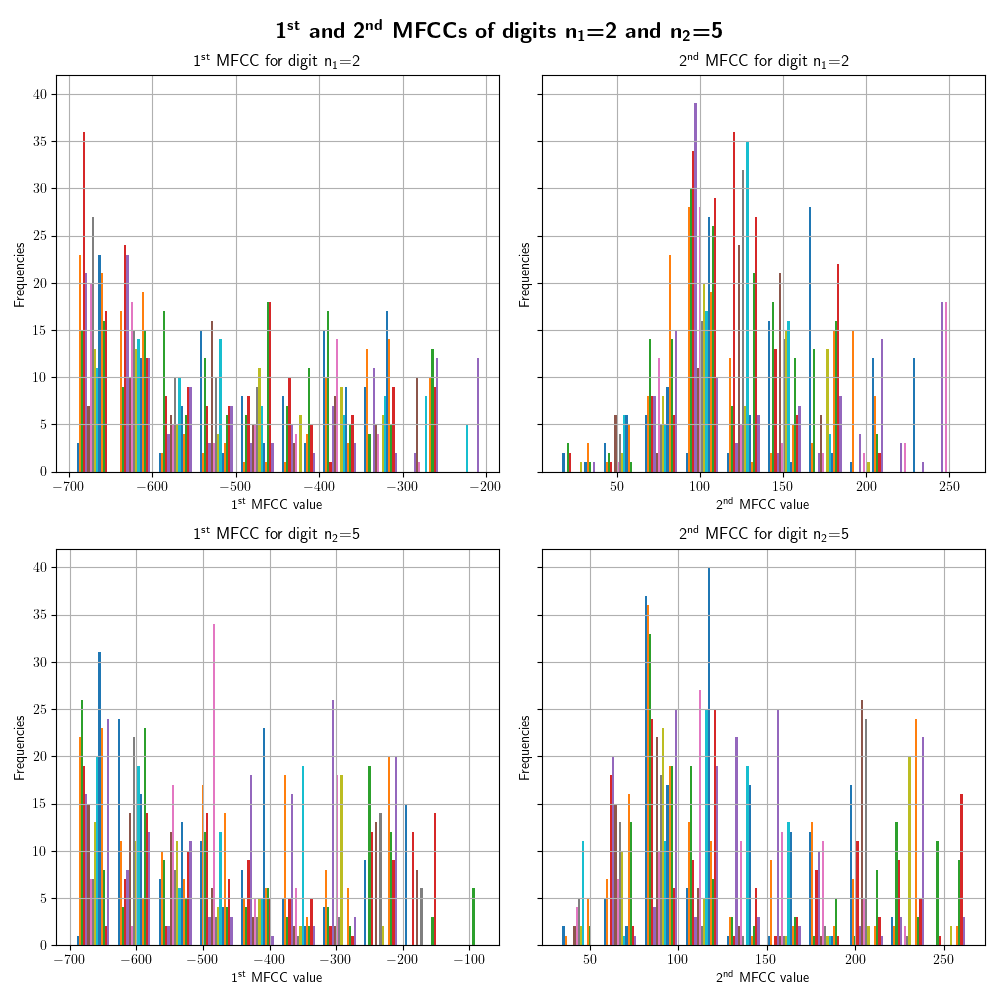
\includegraphics[width=\linewidth]{plots/histograms_step4.png}
\end{figure}

\noindent Αυτό που παρατηρούμε είναι ότι τα MFCC για $n_1=2$ δεν μοιάζουν πολύ μεταξύ τους στο ιστόγραμμα. Αυτό επιβεβαιώνεται και στο επόμενο γράφημα που αναπαριστά τη συσχέτιση μεταξύ τους, καθώς βλέπουμε ότι έχει τιμή 0,03 (γκρι χρώμα), για τον πρώτο ομιλητή. Από την άλλη πλευρά δεν παρατηρούμε το ίδιο για τον δεύτερο ομιλητή, πράγμα μη ευνοϊκό για το consistency της διαχωρισιμότητας των ψηφίων ανάμεσα στους ομιλητές. Αυτή τη παρατήρηση έρχονται να επιβεβαιώσουν και τα ιστογράμματα για $n_2=5$. Σε αυτά βλέπουμε ότι η μορφή τους μοιάζει αλλά και η συσχέτισή τους είναι υψηλή και για τους 2 ομιλητές (κοντά στο 0,85).

\noindent Επιπλέον, όσον αφορά την ικανότητα των MFCC να διαχωρίσουν τα διαφορετικά ψηφία, αυτό που μπορούμε να πούμε διαφάζοντας κατακόρυφα το διάγραμμα είναι ότι τα ιστογράμματα μοιάζουν μεν, δεν είναι πανομοιότυπα δε. Οπότε τα MFCC θα μπορούσαν να είναι η βάση του classification ειδικά εφόσον μετασχηματιστούν σε κάτι άλλο ή από αυτά εξαχθούν ορισμένα στατιστικά χαρακτηριστικά, πράγμα που κάνουμε παρακάτω με την μέση τιμή και την τυπική απόκλισή τους. 

\noindent Στη συνέχεια, υπολογίζουμε τα Mel Filterbank Spectral Coefficients (MFSCs) για δύο εκφωνήσεις των ίδιων ψηφίων από δύο διαφορετικούς ομιλητές και υπολογίζουμε τον πίνακα συνδιακύμανσης τους για κάθε εκφώνηση με την συνάρτηση corrcoef της numpy, παρουσιάζοντας το τελικό αποτέλεσμα σε heatmap της βιβλιοθήκης seaborn.

\begin{figure}[H]
    \centering
    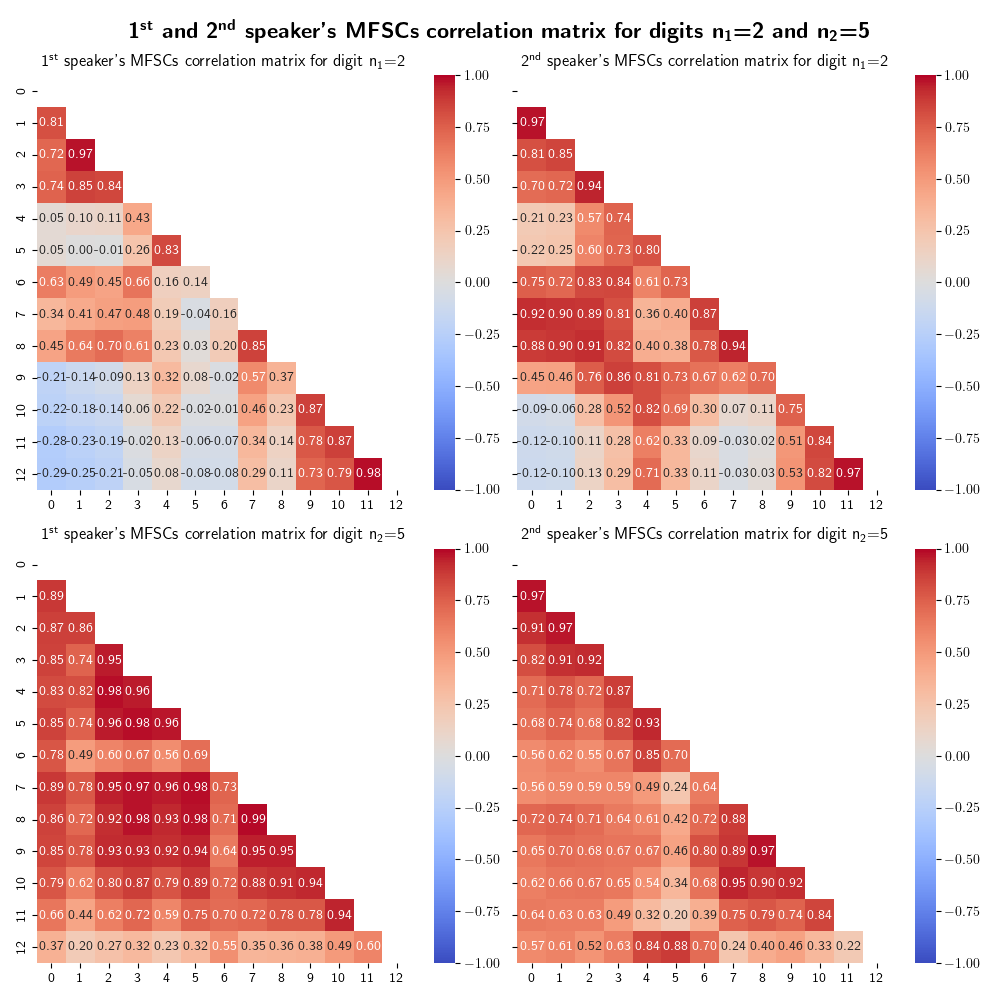
\includegraphics[width=\linewidth]{plots/corrs_mfsc_step4.png}
\end{figure}

\noindent Ύστερα, κάνουμε το ίδιο για τα MFCCs.

\begin{figure}[H]
    \centering
    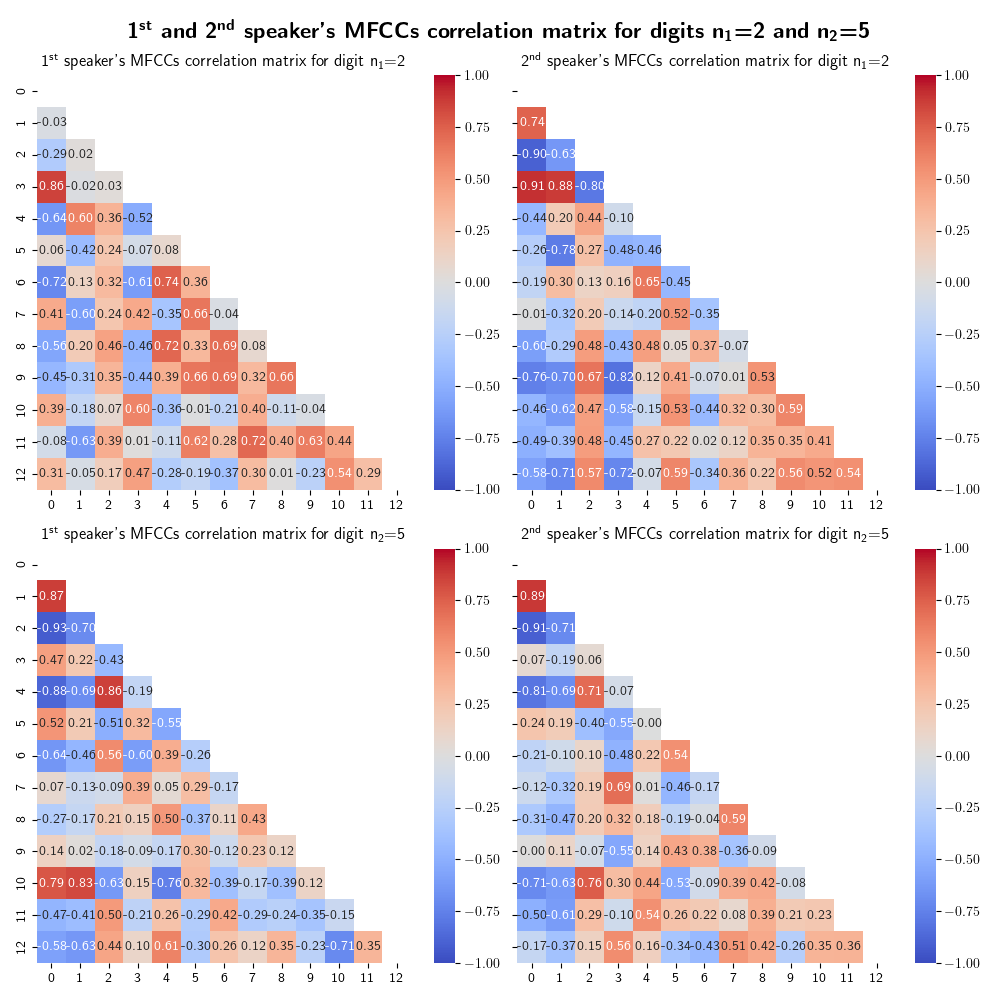
\includegraphics[width=\linewidth]{plots/corrs_mfcc_step4.png}
\end{figure}

\noindent Παρατηρούμε ότι τα MFCCs έχουν πολύ μικρότερη συσχέτιση μεταξύ τους. Για αυτόν τον λόγο, όταν κάνουμε επιλογή χαρακτηριστικών, χρησιμοποιούμε τα MFCCs αντί τα MFSCs, αφού στους περισσότερους αλγορίθμους προτιμάμε τα χαρακτηριστικά μας να είναι κατά το δυνατόν ανεξάρτητα, και το να είναι ασυσχέτιστα είναι προϋπόθεση για αυτό το γεγονός.\\

\noindent Σημειώνουμε ότι τα MSFCs τα λάβαμε με την εντολή \lstinline[language=Python]{librosa.feature.melspectrogram(y=wav, sr=Fs, win_length=win_len, hop_length=step, n_mels=n_features)}.
Ισοδύναμα, θα μπορούσαμε να τα είχαμε λάβει με την εντολή \lstinline[language=Python]{librosa.feature.inverse.mfcc_to_mel(mfcc)}, αφού η βιβλιοθήκη librosa έχει υλοποιημένη την μετατροπή MFCCs σε MFSCs,
ή με την εντολή \lstinline[language=Python]{librosa.db_to_power(scipy.fft.idct(mfcc, type=2, norm="ortho", axis=0))}, αφού τα MFSCs προκύπτουν με τον ίδιο ακριβώς τρόπο με τα MFCCs αλλά χωρίς την εφαρμογή του τελευταίου DFT, οπότε με Inverse DFS μπορούμε να τον αναιρέσουμε και να πάρουμε MFSCs από MFCCs. Την τριπλή αυτή ισοδυναμία επιβεβαιώσαμε και πειραματικά. Προτιμήσαμε τον πρώτο τρόπο, με το melspectrogram εφαρμοσμένο στο wav, γιατί εφαρμόζει τον ευθύ μετασχηματισμό, οπότε δεν υποφέρει από τα επιπλέον αριθμητικά σφάλματα που εισάγουν οι DCT και Inverse DCT.

\section*{Βήμα 5}
Αρχικά χρησιμοποιούμε NumPy για να ενώσουμε όλα τα χαρακτηριστικά του input που έχουμε υπολογίσει (mfcc, delta, delta-deltas) και να φτιάξουμε έναν πίνακα. Κατόπιν υπολογίζουμε για καθένα από αυτά τη μέση τιμή και την τυπική απόκλιση και επιλέγουμε αυτά ως τα τελικά χαρακτηριστικά που θα χρησιμοποιήσουμε για το classification. Στα σχόλια έχουμε το shape των tensors που έχουμε εκτυπώσει για να είμαστε σίγουροι για την ορθότητα των βημάτων μας.

\lstinputlisting[language=Python, firstline=211, lastline=223]{preparation.py}

\noindent Οι 2 πρώτες διαστάσεις που καλούμαστε να παραστήσουμε σε scatter plot είναι οι μέσες τιμές των πρώτων 2 MFCC. To αποτέλεσμα φαίνεται παρακάτω (ο λόγος που χρησιμοποιούμε διαφορετικά χρώματα και σχήματα είναι για να κάνουμε τις κλάσεις μας ευδιάκριτες):

\begin{figure}[H]
    \centering
    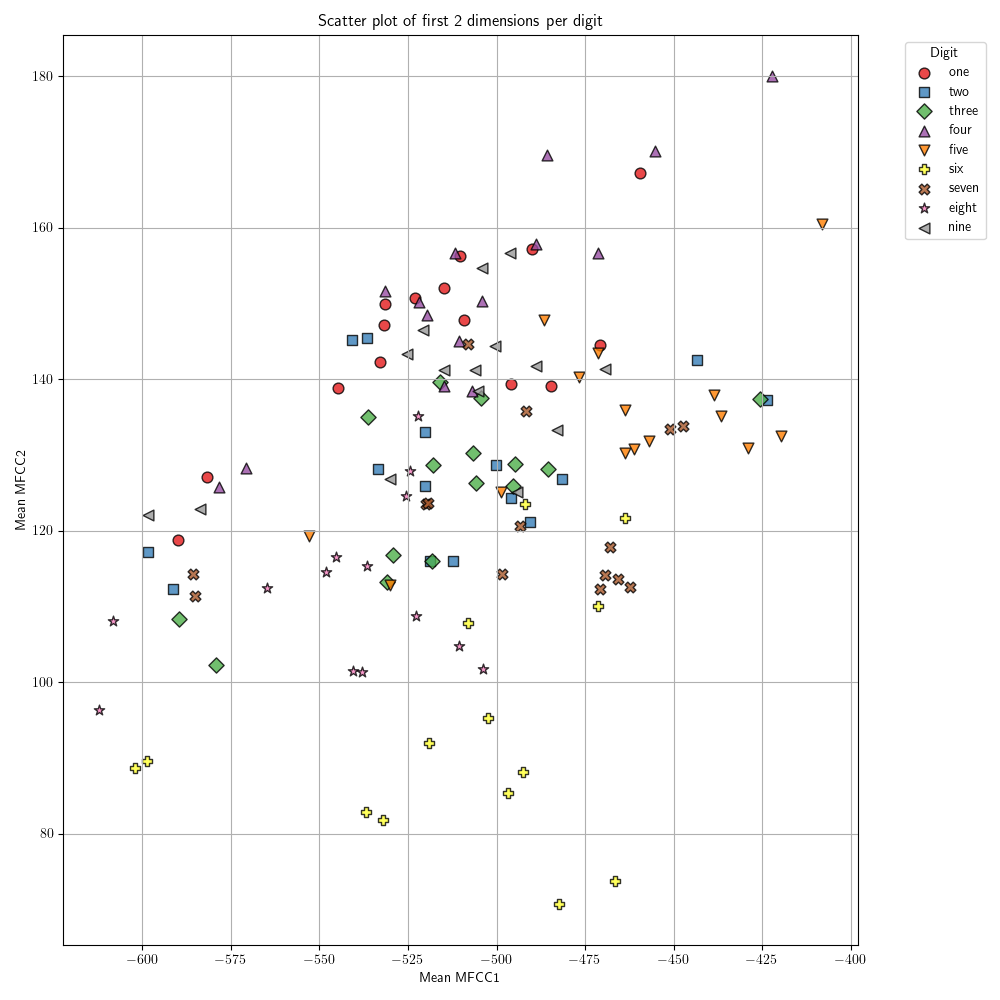
\includegraphics[width=\linewidth]{plots/scatter_plot_2_random_features_step5.png}
\end{figure}

\noindent Ουσιαστικά, αυτό που κάνουμε είναι να βάζουμε 2 "τυχαία" (έστω τα 2 πρώτα) features στο scatter plot για να δούμε ότι οι κλάσεις μας δεν είναι τόσο διαχωρίσιμες. Προετοιμαζόμαστε να συγκρίνουμε το αποτέλεσμα με το PCA στο βήμα 6 όπου τα 2 πρώτα features γίνονται εκείνα που εξηγούν το μεγαλύτερο ποσοστό του variance και έτσι κάνουν τις κλάσεις μας πιο διαχωρίσιμες από αυτό που βλέπουμε παραπάνω.

\section*{Βήμα 6}

Στο βήμα αυτό, εφαρμόζουμε Principal Component Analysis (PCA) για την μείωση διαστατικότητας των δεδομένων. Αρχικά, μειώνουμε τις διαστάεις των διανυσμάτων χαρακτηριστικών σε 2 με την εντολή \lstinline[language=Python]{PCA(n_components=2).fit_transform(feature_vectors)} και στη συνέχεια σε 3 θέτοντας n\_components = 3.\\

\noindent Παρακάτω παραθέτουμε εκ νέου το scatter plot με τις δύο διαστάσεις των μετασχηματισμένων δεδομένων για n\_components = 2.

\begin{figure}[H]
    \centering
    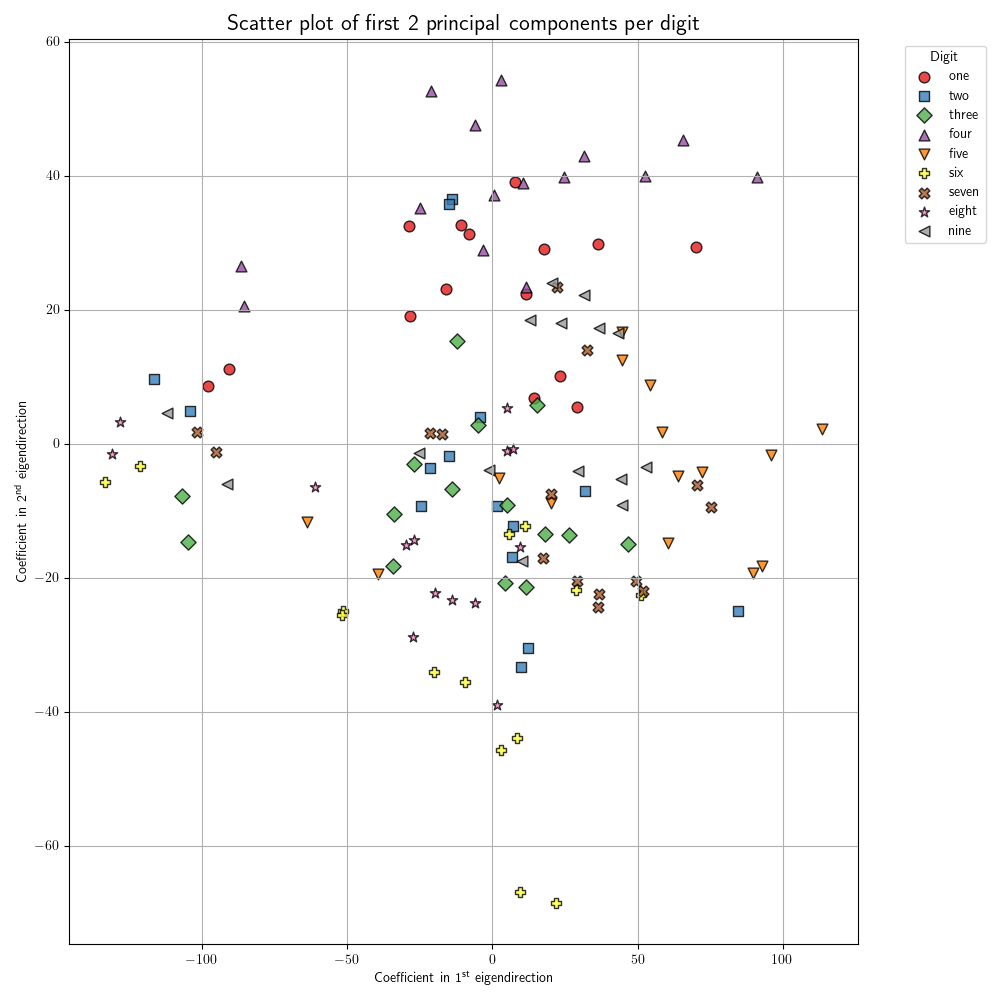
\includegraphics[width=\linewidth]{plots/scatter_plot_2_eigendirections_step6.png}
\end{figure}

\noindent Παρατηρούμε ότι τα σημεία ακόμα δεν είναι ιδιαίτερα διαχωρισμένα, αλλά πολύ περισσότερο από ό,τι στο Βήμα 5 χωρίς PCA. Τα ψηφία είναι καλύτερα μαζεμένα σε περιοχές, αλλά υπάρχουν πολλές επικαλύψεις ακόμα. Το ποσοστό της συνολικής ερμηνευόμενης διασποράς των δεδομένων είναι 70.5\% (άθροισμα στοιχείων πεδίου explained\_variance\_ratio\_).\\

\noindent Ακολούθως, παραθέτουμε το scatter plot με τις τρεις διαστάσεις των μετασχηματισμένων δεδομένων για n\_components = 3.

\begin{figure}[H]
    \centering
    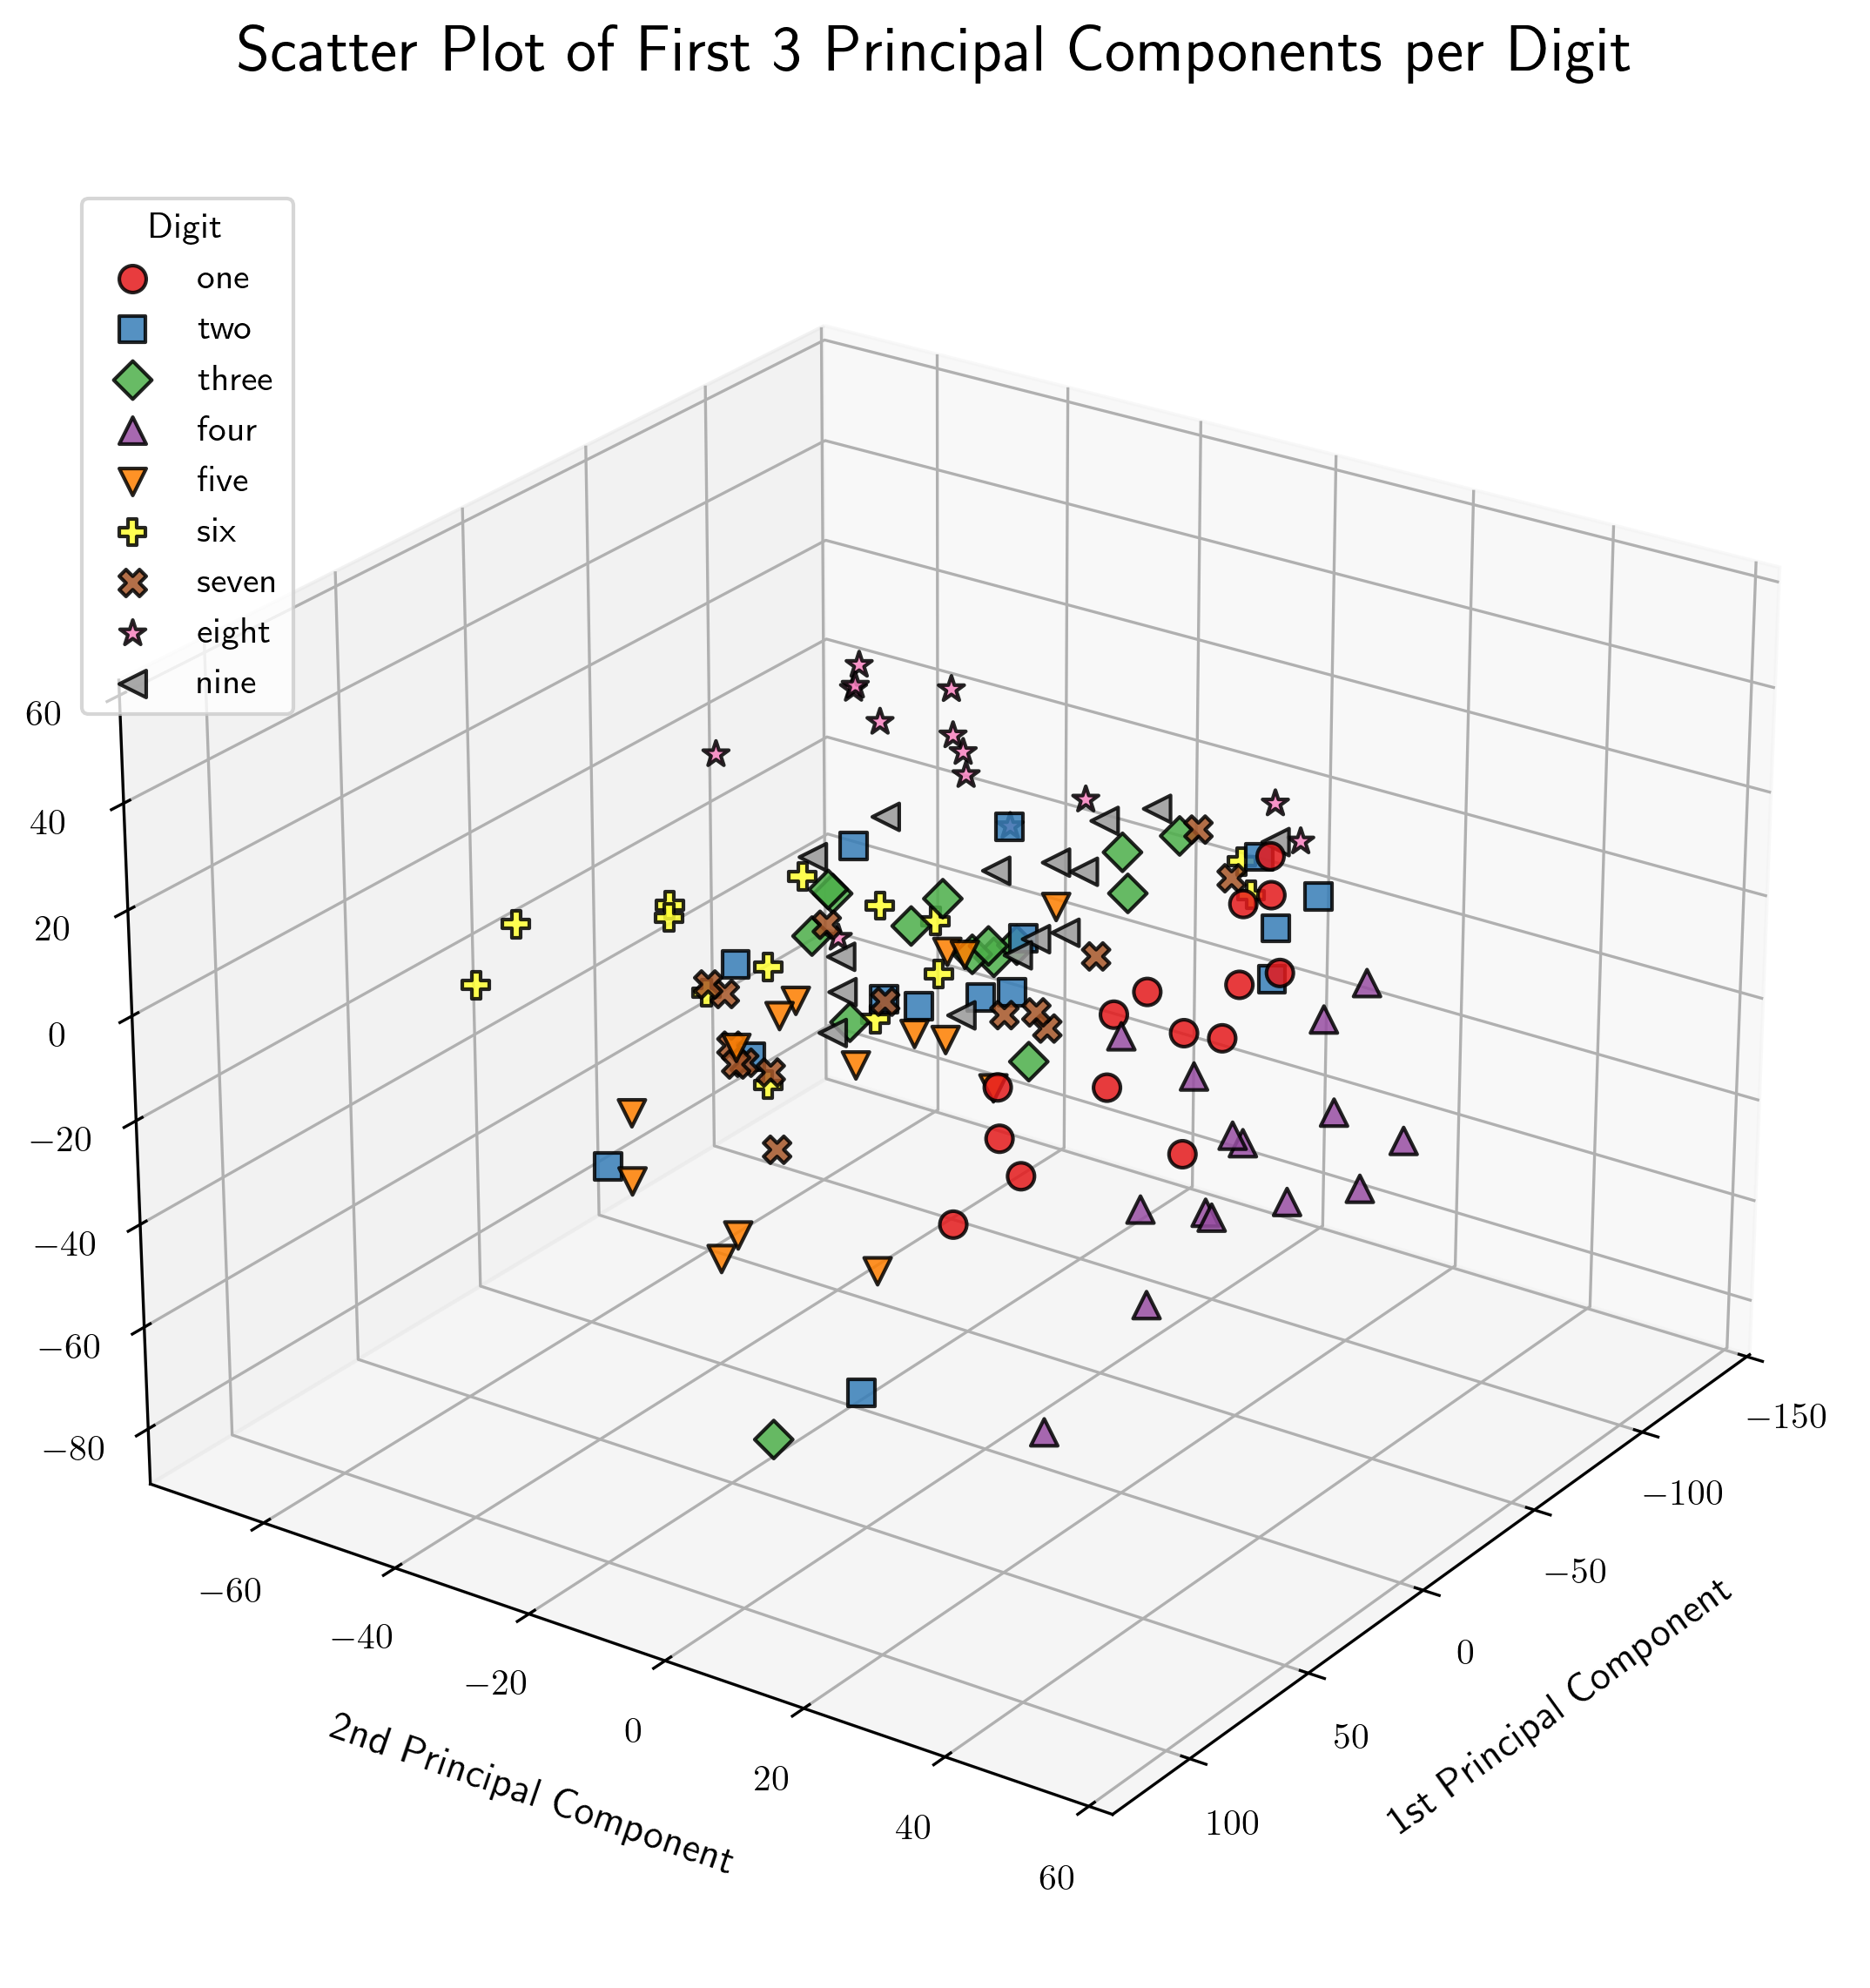
\includegraphics[width=\linewidth]{plots/scatter_plot_3_eigendirections_step6.png}
\end{figure}

\noindent Πλέον, παρατηρούμε ότι τα ψηφία είναι πολύ καλύτερα διαχωρισμένα. Είναι μαζεμένα σε συμπαγείς περιοχές και υπάρχουν πολύ λιγότερες επικαλύψεις, αν και ακόμα υπάρχουν. Επιπλέον, η συνολική ερμηνευόμενη διασπορά είναι 81.4\%. Ακόμα, το πεδίο explained\_variance\_ratio\_ μας δίνει το ποσοστό της ερμηνευόμενης διασποράς από κάθε συνιστώσα του PCA, δηλαδή τη διασπορά σε στον κάθε άξονα των πρώτων ιδιοδιανυσμάτων του πίνακα συνδιασποράς. Αυτή είναι πολύ μεγάλη για το πρώτο διάνυσμα και μονότονα μειώνεται όσο αυξάνονται οι συνιστώσες.\\

\noindent Μπορούμε να θεωρήσουμε ότι η μείωση διαστατικότητας ήταν επιτυχημένη, αφού ερμηνεύσαμε το 70.5\% και 81.4\% με μόνο 2 και 3 συνιστώσες αντίστοιχα, αλλά για να έχουμε ακόμα καλύτερη απόδοση, θα βοηθούσε να έχουμε λίγες ακόμα συνιστώσες ώστε να ερμηνεύσουμε ακόμα μεγαλύτερο τμήμα της διασποράς και να διαχωριστούν πλήρως τα δεδομένα.

\section*{Βήμα 7}

Στο βήμα αυτό, αρχικά χωρίζουμε τα δεδομένα μας σε δεδομένα εκπαίδευσης (train, 70\%) και δεδομένα ελέγχου (test, 30\%) με χρήση της συνάρτησης train\_test\_split. Προτού δοκιμάσουμε οποιοδήποτε μοντέλο κανονικοποιούμε τα δεδομένα για να τα χειρίζονται "δίκαια" μέθοδοι επιλογής χαρακτηριστικών όπως η PCA (που χρησιμοποιούμε ξανά) και μοντέλα ταξινόμησης που βασίζονται σε μετρικούς χώρους.\\

\noindent Ακολούθως, σε όλα τα μοντέλα μας θα δοκιμάζουμε ως υπερπαράμετρο το πλήθος συνιστωσών του PCA, από 2 έως και 10. Όλα τα μοντέλα θα αξιολογούνται στο τέλος με βάση το accuracy και το F1-score. Το F1-score το χρησιμοποιούμε κυρίως σε περιπτώσεις που υπάρχουν ανισορροπίες στην εκπροσώπηση των κλάσεων στα δεδομένα, κάτι που παρατηρούμε ότι εδώ δεν συμβαίνει. Για αυτό, σε όλα τα μοντέλα που εξετάζουμε, το accuracy και το f1-score είναι πολύ κοντά και έχουν την ίδια τάση.\\

\noindent Το πρώτο μοντέλο που δοκιμάζουμε είναι ο Naive Bayes για Γκαουσιανές τυχαίες μεταβλητές (\lstinline[language=Python]{GaussianNB()}). Παραθέτουμε το διάγραμμα των μετρικών ως προς το πλήθος συνιστωσών κατά το PCA. Το καλύτερο μοντέλο λήφθηκε για 10 συνιστώσες με ακρίβεια 60\%.

\begin{figure}[H]
    \centering
    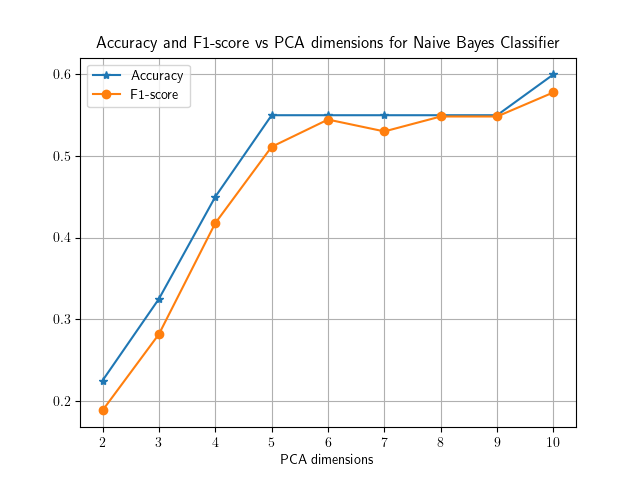
\includegraphics[width=\linewidth]{plots/accuracies_and_f1_naive_bayes_step7.png}
\end{figure}

\noindent Το δεύτερο μοντέλο που δοκιμάζουμε είναι το Support Vector Machine με το μη γραμμικό απειροδιάστατο RBF kernel (\lstinline[language=Python]{SVC()}). Παραθέτουμε και εδώ το αντίστοιχο διάγραμμα. Το καλύτερο μοντέλο λήγθηκε πάλι για 10 συνιστώσες με ακρίβεια 60\%.

\begin{figure}[H]
    \centering
    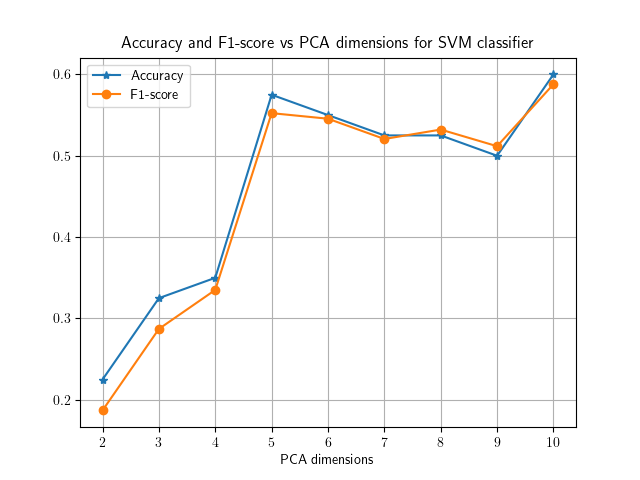
\includegraphics[width=\linewidth]{plots/accuracies_and_f1_svm_step7.png}
\end{figure}

\noindent Το τρίτο μοντέλο που δοκιμάζουμε είναι το k-Nearest Neigbors, με επιπλέον υπερπαράμετρο το $k \in \{1, 3, 5, 7\}$ (\lstinline[language=Python]{KNeighborsClassifier(n_neighbors=k)}). Παραθέτουμε το αντίστοιχο τριδιάστατο διάγραμμα. Το καλύτερο μοντέλο λήφθηκε για 10 συνιστώσες και k = 5 με ακρίβεια 70\%.

\begin{figure}[H]
    \centering
    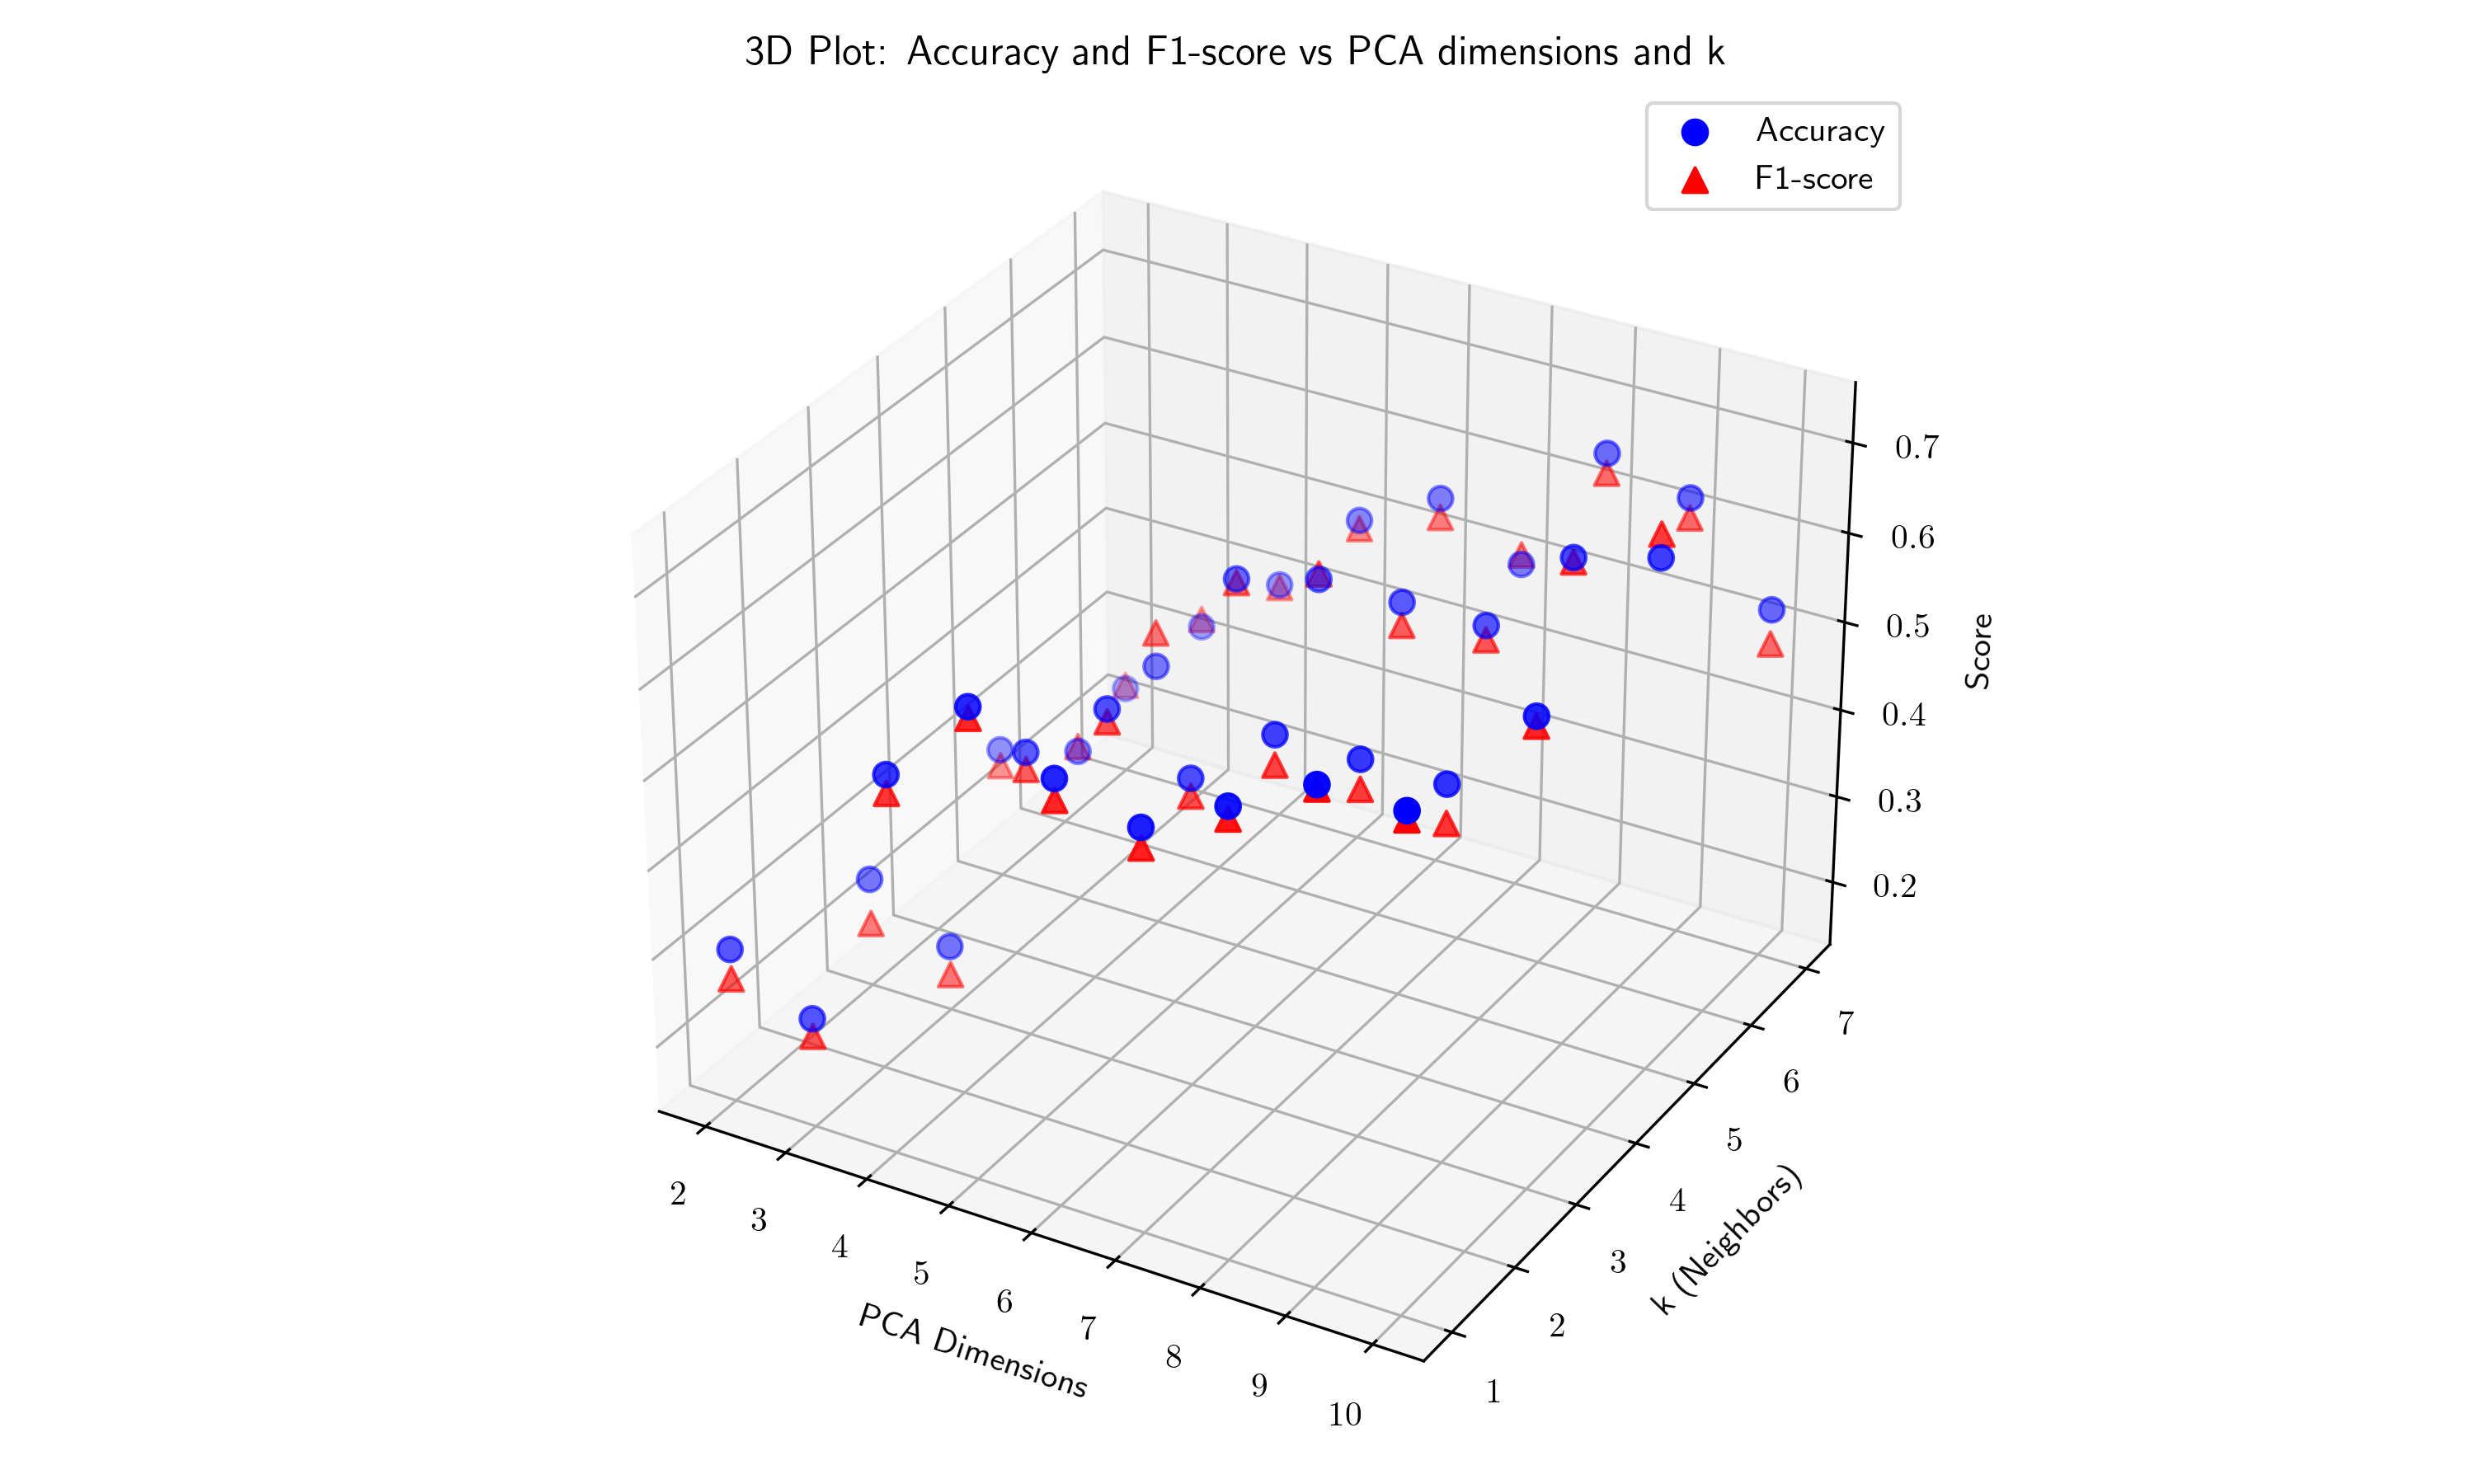
\includegraphics[width=\linewidth]{plots/3D_accuracy_f1_knn_step7.png}
\end{figure}

\noindent Το τελευταίο μοντέλο που δοκιμάζουμε είναι το Logistic Regression (\lstinline[language=Python]{LogisticRegression()}). Παραθέτουμε πάλι το αντίστοιχο διάγραμμα. Το καλύτερο μοντέλο λήφθηκε για 6 συνιστώσες με ακρίβεια 65\%.

\begin{figure}[H]
    \centering
    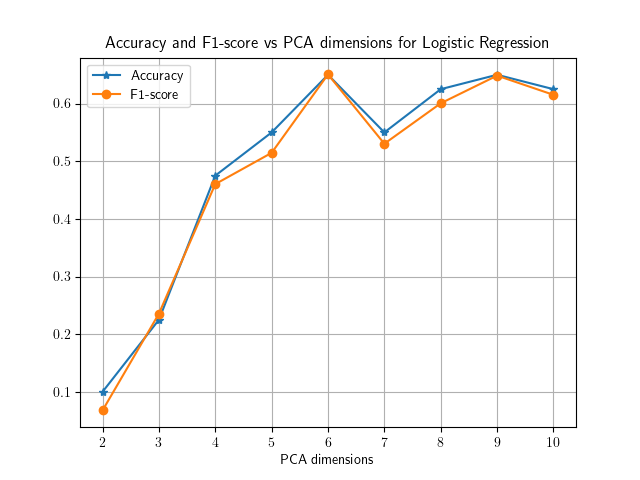
\includegraphics[width=\linewidth]{plots/accuracies_and_f1_lr_step7.png}
\end{figure}

\section*{Βήμα 8}
Σε αυτό το βήμα μας ζητείται να δημιουργήσουμε ακολουθίες 10 σημείων ενός ημιτόνου και ενός συνημιτόνου συχνότητας 40Hz. Στόχος είναι να προβλέψουμε τις ακολουθίες συνημιτόνου έχοντας ως δεδομένες εκείνες των ημιτόνων. \\

\noindent Για να το πετύχουμε αυτό επιστρατεύουμε 3 είδη νευρωνικών δικτύων, το RNN, το LSTM και το GRU. Για να τα ορίσουμε και να τα εκπαιδεύσουμε αξιοποιούμε την PyTorch.

\begin{itemize}
    \item \textbf{RNN:} Πρόκειται για ένα τύπο νευρωνικού δικτύου ειδικά σχεδιασμένου ώστε να επεξεργαστούμε ακολουθιακά δεδομένα και να ανιχνεύσουμε τις εξαρτήσεις τους και τα μοτίβα τους στο χρόνο.

        \begin{figure}[h]
            \centering
            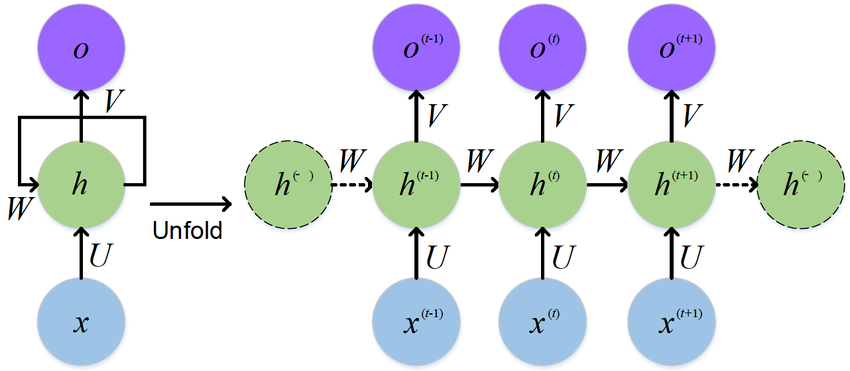
\includegraphics[width=0.5\linewidth]{plots/rnn.png}
        \end{figure}

        Ο κώδικας του ορισμού του είναι ο εξής: \\
        \lstinputlisting[language=Python]{scripts/rnn.py} 
        
        Ουσιαστικά έχουμε το component που υλοποιοεί ένα RNN, το οποίο πρσφέρεται έτοιμο από την PyTorch και κατόπιν ένα fully connected layer το οποίο συνδυάζει τα outputs των hidden layers του RNN κάθε χρονική στιγμή-δείγμα και μας δίνει το τελικό προβλεπόμενο output για τη δεδομένη χρονική στιγμή. 

    \item \textbf{LSTM:} Το LSTM είναι ένα είδος RNN το οποίο αναπτύχθηκε προκειμένου να αντιμετωπίσει το πρόβλημα του vanishing gradient που εμφανιζόταν έντονα στον πρόγονό του. Ουσιαστικά, δίνει δυνατότητα short term memory στο μοντέλο ώστε να "θυμάται" πληροφορίες και εξαρτήσεις στα δεδομένα για χιλιάδες δείγματα, σε αντίθεση με το RNN το οποίο "έχανε" τις εξαρτήσεις δεδομένων που απείχαν κάποιο μεγάλο αριθμό δειγμάτων (αυτό είναι το manifestation του vanishing gradient).

        \begin{figure}[h]
            \centering
            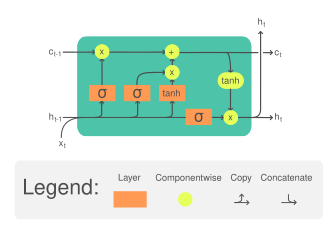
\includegraphics[width=0.5\linewidth]{plots/lstm.png}
        \end{figure}

        Ο κώδικας του ορισμού του φαίνεται παρακάτω και ακολουθεί τη λογική του RNN: \\
        \lstinputlisting[language=Python]{scripts/lstm.py}

    \item \textbf{GRU:} Είναι και αυτό "απόγονος" του RNN. Πρακτικά μοιάζει με το LSTM, μόνο που έχει έναν μηχανισμό από πύλες στο input, αλλά δεν έχει πύλη στο output και συνεπώς έχει λιγότερες παραμέτρους από το LSTM. 

        \begin{figure}[h]
            \centering
            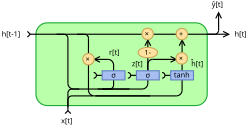
\includegraphics[width=0.5\linewidth]{plots/gru.png}
        \end{figure}

        Ο κώδικας του ορισμού του φαίνεται παρακάτω και ακολουθεί τη λογική του RNN και του LSTM: \\
        \lstinputlisting[language=Python]{scripts/gru.py}
\end{itemize}

\noindent Στην συνέχεια, εκπαιδεύουμε τα μοντέλα μας και συγκρίνουμε την απόδοσή τους. Η διαδικασία που ακολουθούμε είναι η εξής:

\begin{enumerate}
    \item \textbf{Δημιουργία δειγμάτων ημιτόνων και συνημιτόνων:} \\
    Με την NumPy δημιουργόυμε τα σήματα-εισόδους για τα νευρωνικά δίκτυα μας καθώς και τα σήματα-στόχους που θέλουμε να προβέψουμε (t = np.linspace(0, 1, total\_points),
    x = np.sin(2*np.pi*f*t), y = np.cos(2*np.pi*f*t))

    \item \textbf{Εκπαίδευση των μοντέλων:} \\
    \lstinputlisting[language=Python]{scripts/trainning.py}

    Ως κριτήριο ελαχιστοποίησης επιλέξαμε το Mean Square Error ενώ για optimizer τον Adam. O Adam ενσωματώνει και όρους ορμής στην δική του υλοποίηση του gradient descend. Εκπαιδεύουμε όλα τα μοντέλα για 100 εποχές. \\
    Αρχικά, πριν από κάθε εποχή πρέπει να καθαρίσουμε τα προηγούμενα gradients γιατί η default συμπεριφορά της PyTorch είναι να τα συσσωρεύει, όχι να τα πανωγράφει. \\
    Στη συνέχεια, υπολογίζουμε το output του μοντέλου και το loss (αντίστοιχο της απόκλισης από το στόχο μας). Τέλος κάνουμε backpropagation τα loss gradients και ενημερώνουμε τα βάρη. \\
    Τα losses αποθηκεύονται ώστε να χρησιμοποιηθούν σε διαγράμματα μετέπειτα.

    \item \textbf{Αξιολόγηση των μοντέλων:} \\
    \lstinputlisting[language=Python]{scripts/eval.py}
    Αρχικά, βάζουμε το μοντέλο σε eval mode (από documentation της PyTorch) και κατόπιν απενεργοποιούμε τον υπολογισμό και την αποθήκευση των gradients διότι αυτή η υπολογιστικά ακριβή διαδικασία δεν είναι απαραίτητη κατά το inference. Τέλος υπολογίζουμε τις μετρικές μας για τα test samples και τις επιστρέφουμε.
\end{enumerate}

\subsection*{Αποτελέσματα}

\begin{figure}[h]
    \centering
    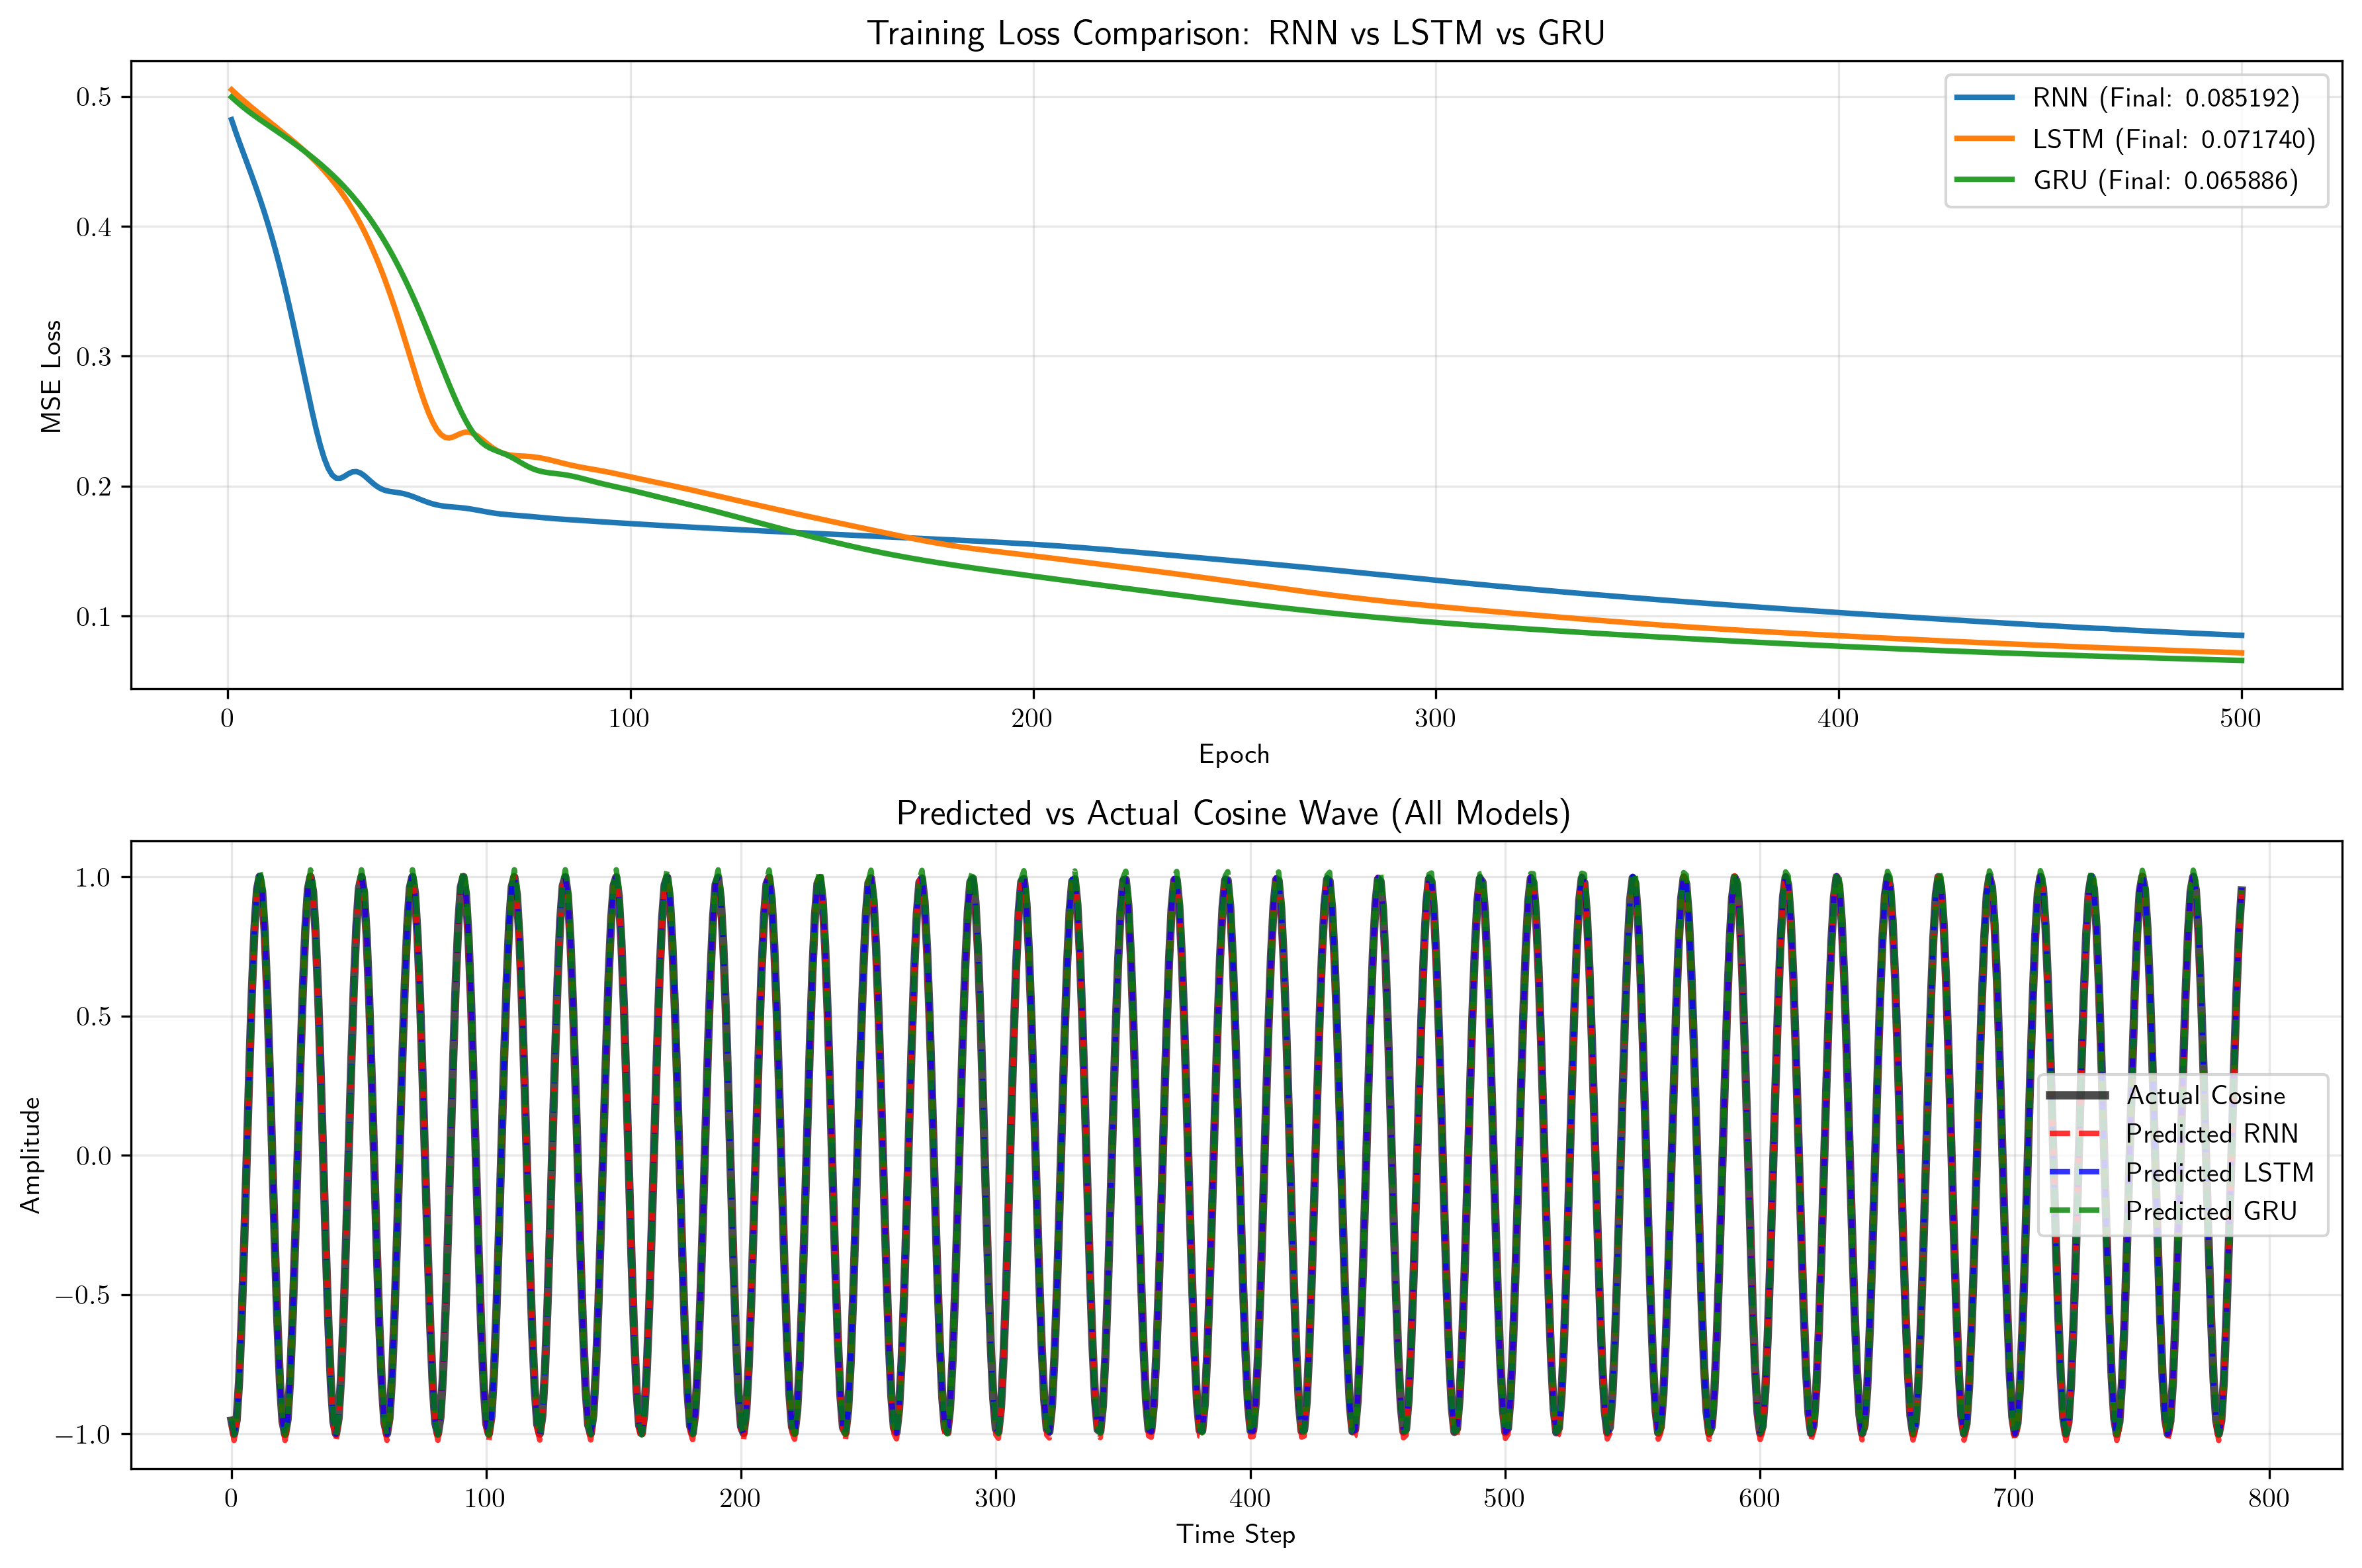
\includegraphics[width=0.9\linewidth]{plots/final_all_models_comparison.png}
\end{figure}

\noindent Σε αυτό το γράφημα εξετάζουμε τη συμπεριφορά των μοντέλων κατά την εκπαίδευσή τους και παίρνουμε μια πρώτη εικόνα για το κατά πόσο το αποτέλεσμα είναι ικανοποιητικό. \\

\noindent Βλέπουμε ότι έχουμε εκπαιδεύσει τα μοντέλα μας για 500 εποχές. Καταλήξαμε σε αυτή την επιλογή ως εξής:

\begin{enumerate}
    \item Αρχικά, εκπαιδεύσαμε με 100 εποχές. Αυτό οδήγησε στο εξής παράδοξο: Το RNN, θεωρητικά το πιο "αδύναμο" μοντέλο είχε το μικρότερο loss - δηλαδή είχε προσαρμοστεί καλύτερα στα δεδομένα. Αυτό μπορεί να έχει μόνο μία εξήγηση, δεδομένου ότι έχει μικρότερη χωρητικότητα από τα προηγούμενα 2. Ο μεγαλύτερος αριθμός παραμέτρων των LSTM και GRU δεν τους έχει επιτρέψει να συγκλίνουν ακόμα. Οπότε αυξάνουμε τον αριθμό εποχών σε 300.

    \item Όπως φαίνεται και στο plot παραπάνω, μετά τις 180 εποχές πράγματι τόσο το LSTM όσο και το GRU έχουν μικρότερο loss από το RNN. Αλλά βλέπουμε ότι το loss έχει την τάση να μειωθεί κι άλλο. Οπότε αυξάνουμε σε 500 εποχές

    \item Βλέπουμε ότι το loss δεν βελτιώνεται οπότε σταματάμε (σε αυτό το σημείο θα μπορούσαμε να αρχίσουμε να αυξάνουμε τα hidden layers).
\end{enumerate}

\noindent Αφότου εξηγήσαμε την διαδικασία της εκπαίδευσής μας, βλέπουμε ότι και το αποτέλεσμα για τα μοντέλα μας, οπτικά, είναι αρκετά υποσχόμενο. Για να το επιβεβαιώσουμε πλήρως εξετάζουμε το αποτέλεσμα σε ένα zoom της κυματομορφής για κάθε μοντέλο ξεχωριστά.

\begin{figure}[H]
    \centering
    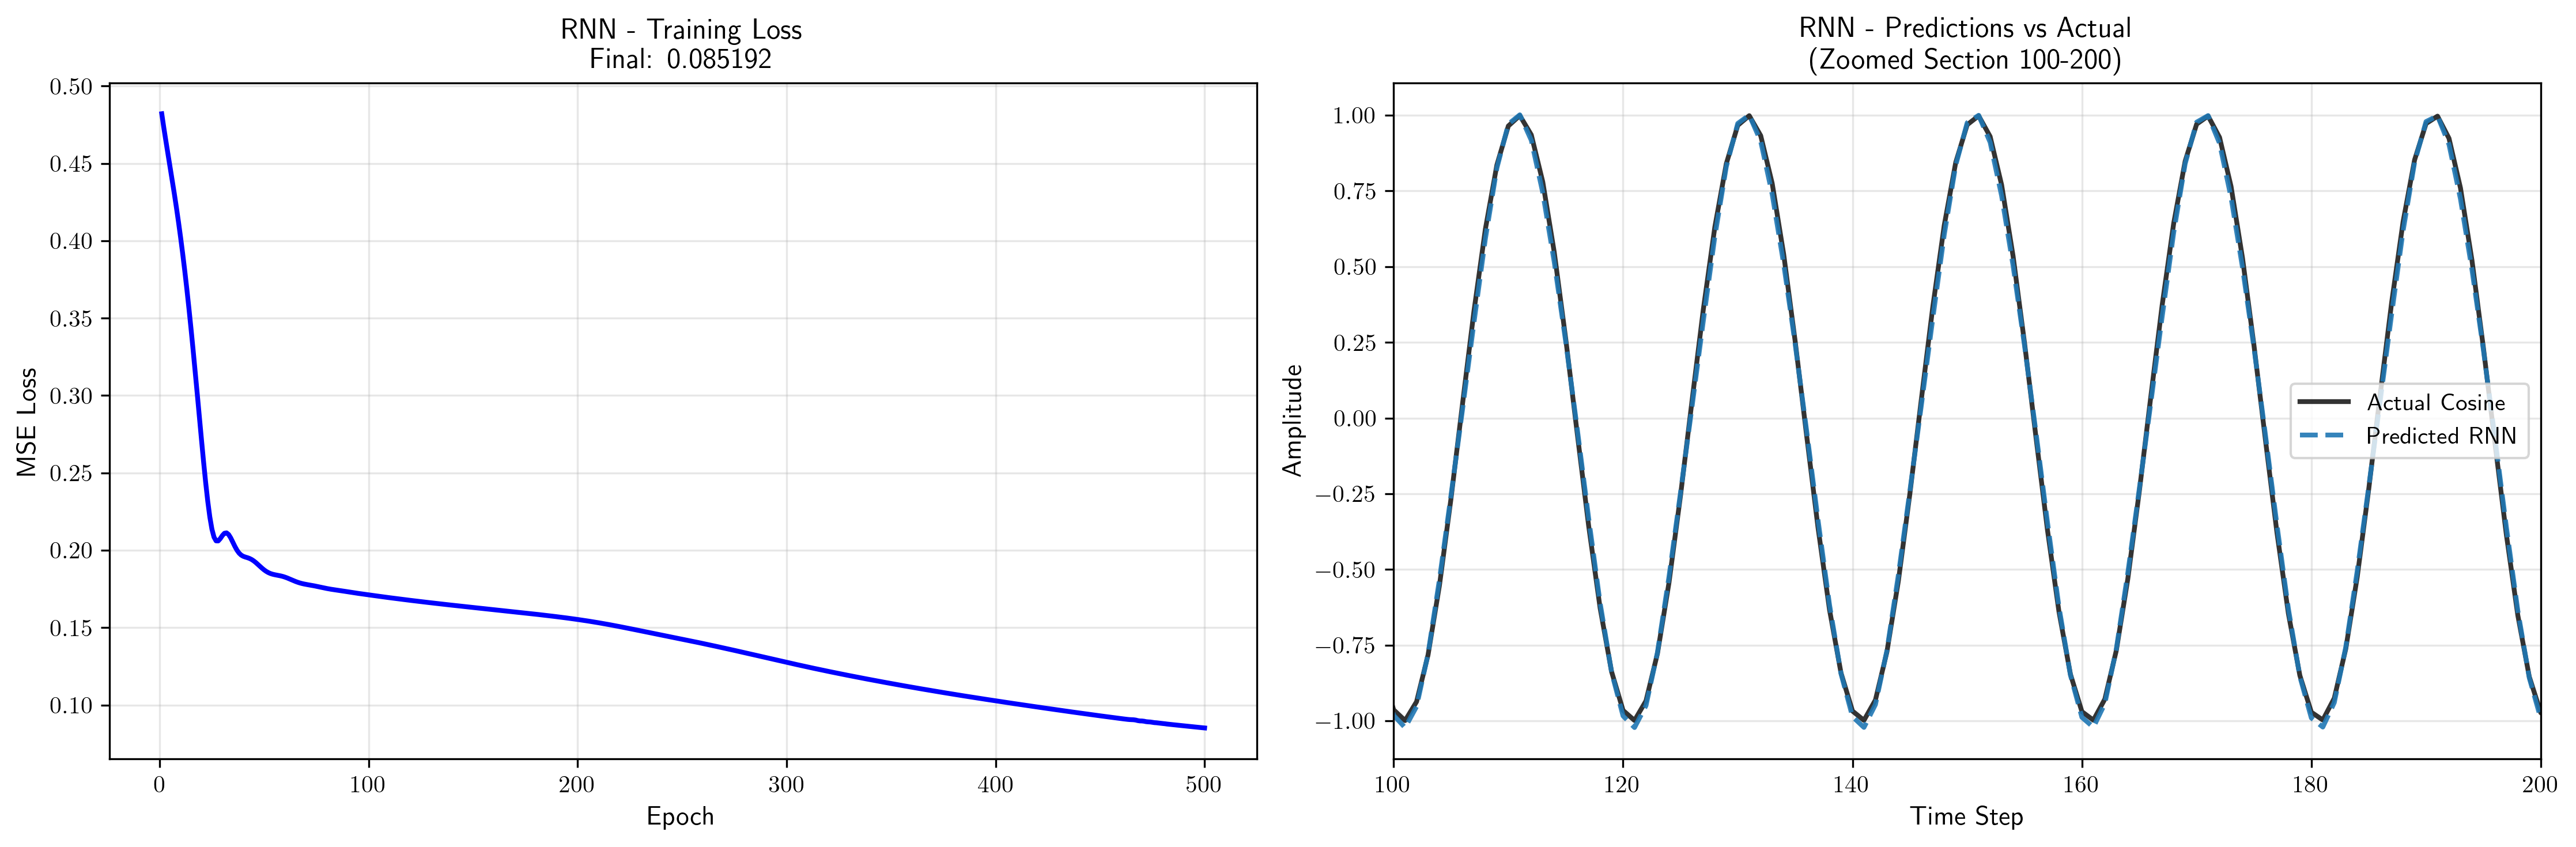
\includegraphics[width=0.9\linewidth]{plots/rnn_clean.png}
\end{figure}

\begin{figure}[H]
    \centering
    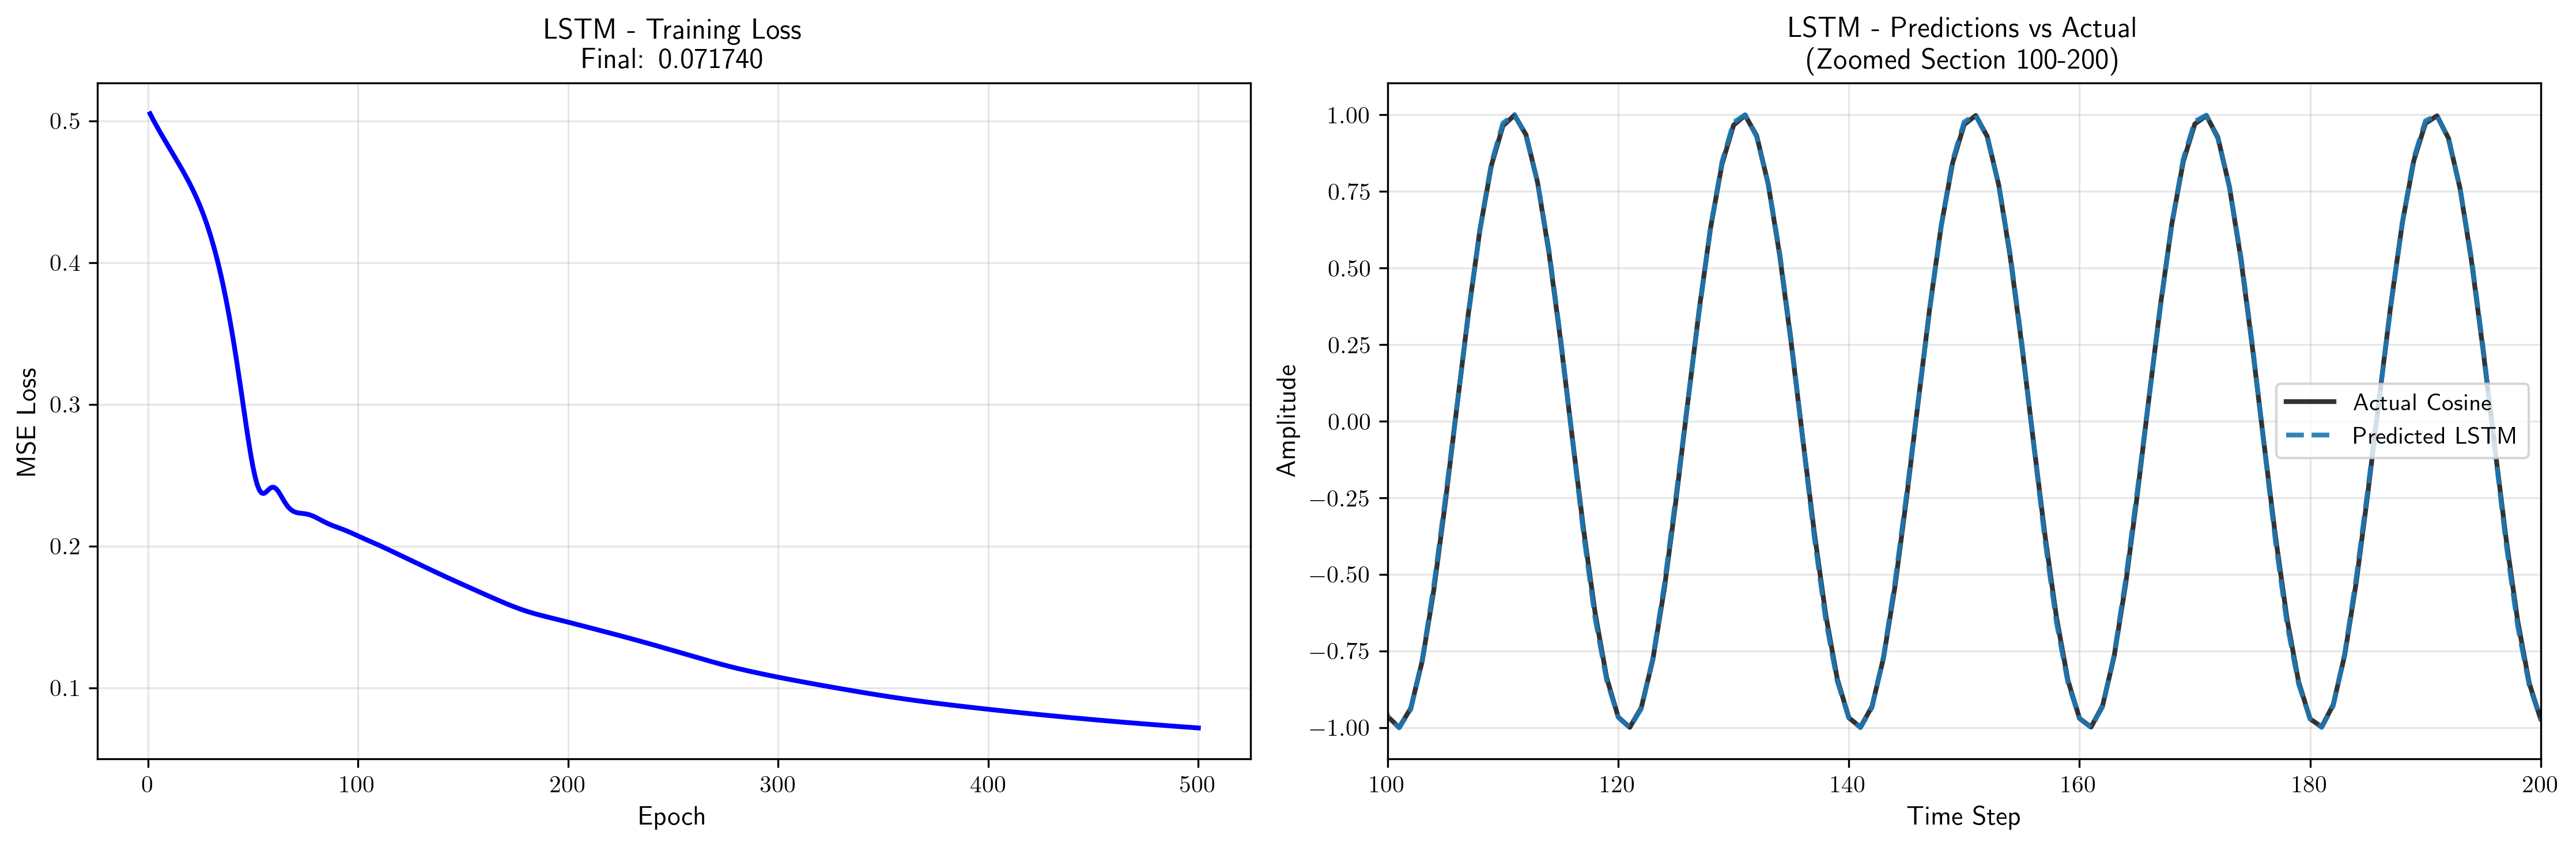
\includegraphics[width=0.9\linewidth]{plots/lstm_clean.png}
\end{figure}

\begin{figure}[H]
    \centering
    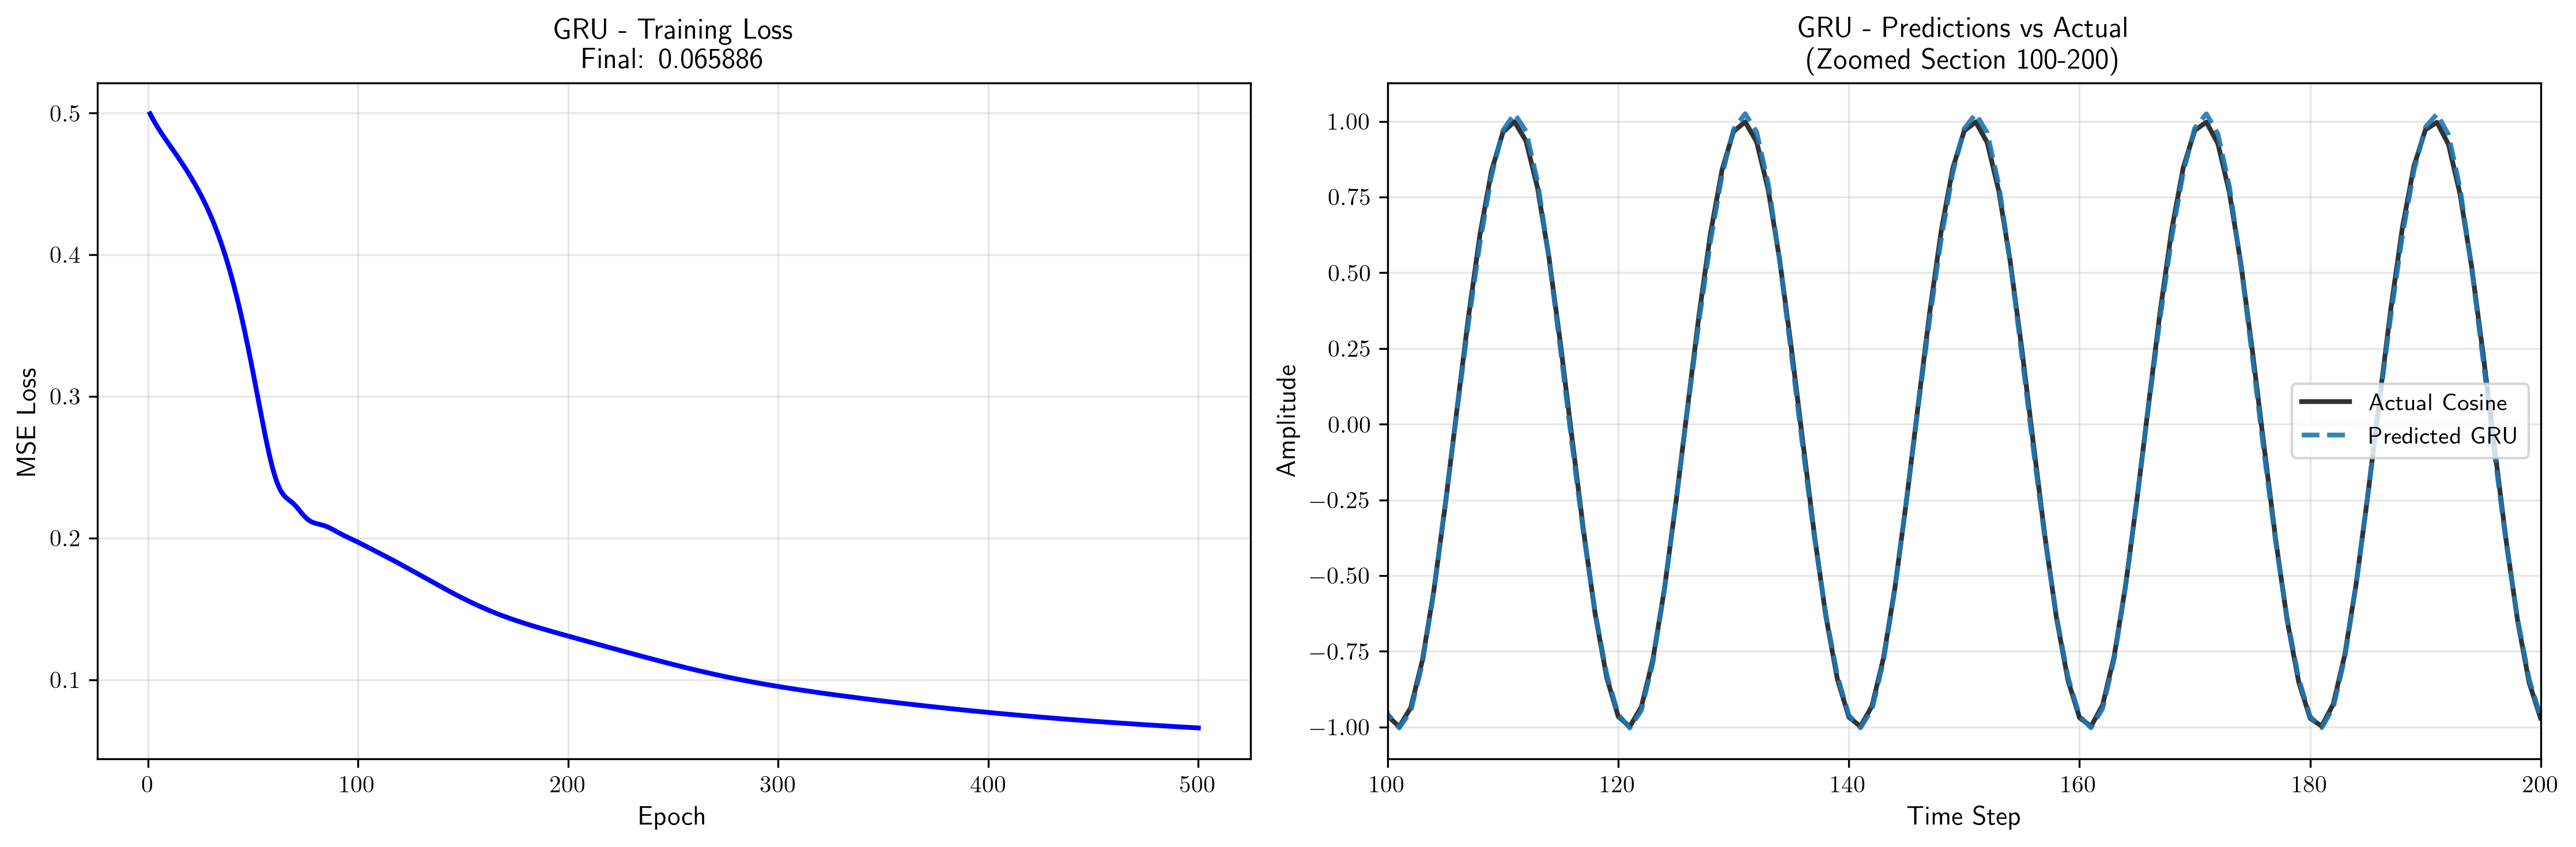
\includegraphics[width=0.9\linewidth]{plots/gru_clean.png}
\end{figure}

\noindent Και για τα 3 μοντέλα το αποτέλεσμα είναι πολύ ικανοποιητικό. \\

\noindent Τέλος, επιλέγουμε το καλύτερο μοντέλο με βάση το μικρότερο MSE στο test set. Αυτό βλέπουμε ότι είναι το GRU.

\begin{figure}[H]
    \centering
    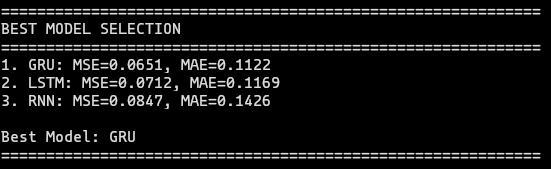
\includegraphics[width=0.5\linewidth]{plots/best_model_selection.png}
\end{figure}

\section*{Βήμα 9}

Πρώτα από όλα κάνουμε clone τα δεδομένα σε μορφή .wav από το repository της εργασίας στον υπολογιστή μας. \\

\noindent Κατόπιν, υλοποιούμε τη συνάρτηση \textit{parse\_free\_digits} προκειμένου να διαβάσουμε σωστά τα αρχεία με τη βιβλιοθήκη librosa.

\lstinputlisting[language=Python, firstline=5, lastline=26]{../../lab.py}

\noindent Το αποτέλεσμα της κλήσης της συνάρτησης είναι:

\begin{center}
	\textbf{Total wavs: 3000. Fs = 8000 Hz}
\end{center}

\noindent Στην συνέχεια βασισμένοι στην υπολοποίηση του βοηθητικού κώδικα ορίζουμε τη δικιά μας συνάρτηση \textit{split\_free\_digits} την οποία παρουσιάζουμε παρακάτω:

\lstinputlisting[language=Python, firstline=27, lastline=61]{../../lab.py}

\noindent Τρέχουμε τον κώδικα για να επιβεβαιώσουμε την ορθή λειτουργία του:

\begin{figure}[H]
	\centering
	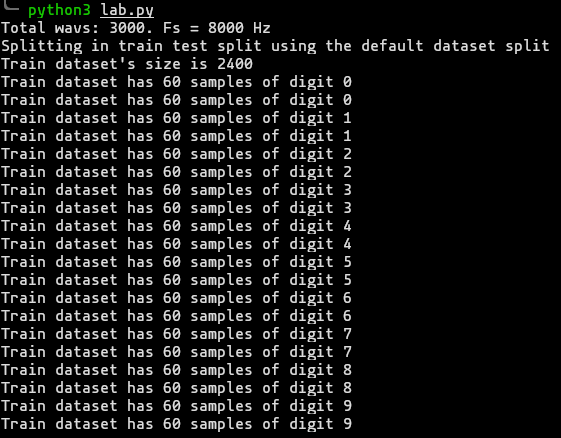
\includegraphics[width=0.5\linewidth]{plots/train_test_res.png}
\end{figure}

\noindent Βλέπουμε ότι το split που έχουμε κάνει έχει μέγεθος 2400, δηλαδή είναι πράγματι το 80\% του 3000. Επιπλέον, είναι ισορροπημένο, αφού υπάρχει ίδιος αριθμός δειγμάτων ήχου σε κάθε κατηγορία - ψηφίο (60). Επομένως ως μετρική του \textit{accuracy} θα είναι αρκετό για να αξιολογήσουμε την επίδοση των ταξινομητών μας (όπως είδαμε και στην προπαρασκευή, στην περίπτωση του ισορροπημένου dataset το F1-score ακολουθεί το ίδιο trend με το accuracy). \\

\noindent Αφού επιβεβαιώσαμε την ορθή λειτουργία της ρουτίνας μας αφαιρούμε - μετατρέπουμε σε σχόλιο τον κώδικα για το debugging.

\section*{Βήμα 10}


\bibliographystyle{plain}
\bibliography{bibliography}

\end{document}